%\lstinputlisting[language=bash,basicstyle=\small]{python_codes/fieldstone_78/keywords.ascii}

\begin{center}
Code at \url{https://github.com/cedrict/fieldstone/tree/master/python_codes/fieldstone_78}
\end{center}

\par\noindent\rule{\textwidth}{0.4pt}

%%%%%%%%%%%%%%%%%%%%%%%%%%%%%%%%%%%%%%%%%%%%%%%%%%%%%%%%%%%%%%%%%%%%%%%%%%%%%%%%%%%%%%%%%%%%%%%%%%%%


Although the $Q_1\times P_0$ is not LBB-stable (see Section~\ref{MMM-ss:LBBcond})
it has been proven that some spatial arrangements of this element can be, such as the
so-called Stenberg macro-element described in Section~\ref{MMM-ss:meshtopos}.
I have gathered 7 mesh types from the literature and they are shown 
here under: 

\begin{center}
0)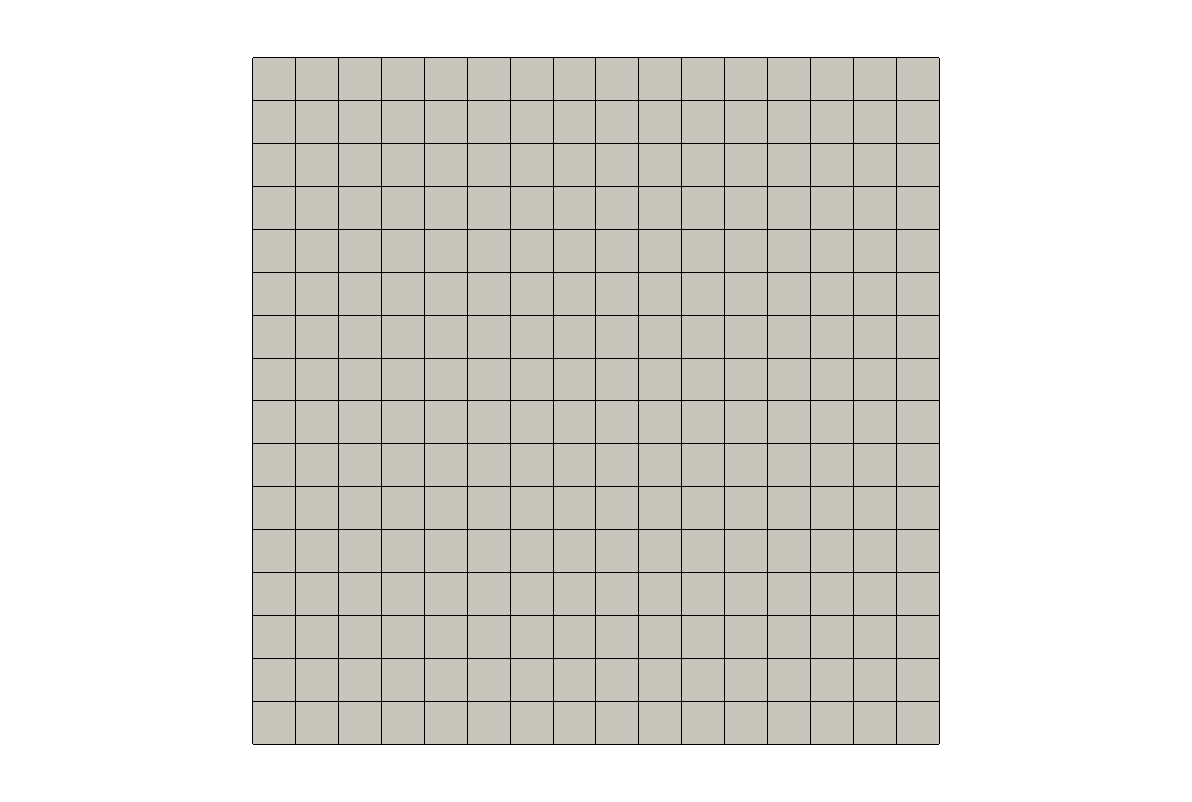
\includegraphics[width=4cm]{python_codes/fieldstone_78/results/mms_dh/16x16/grid0000}
1)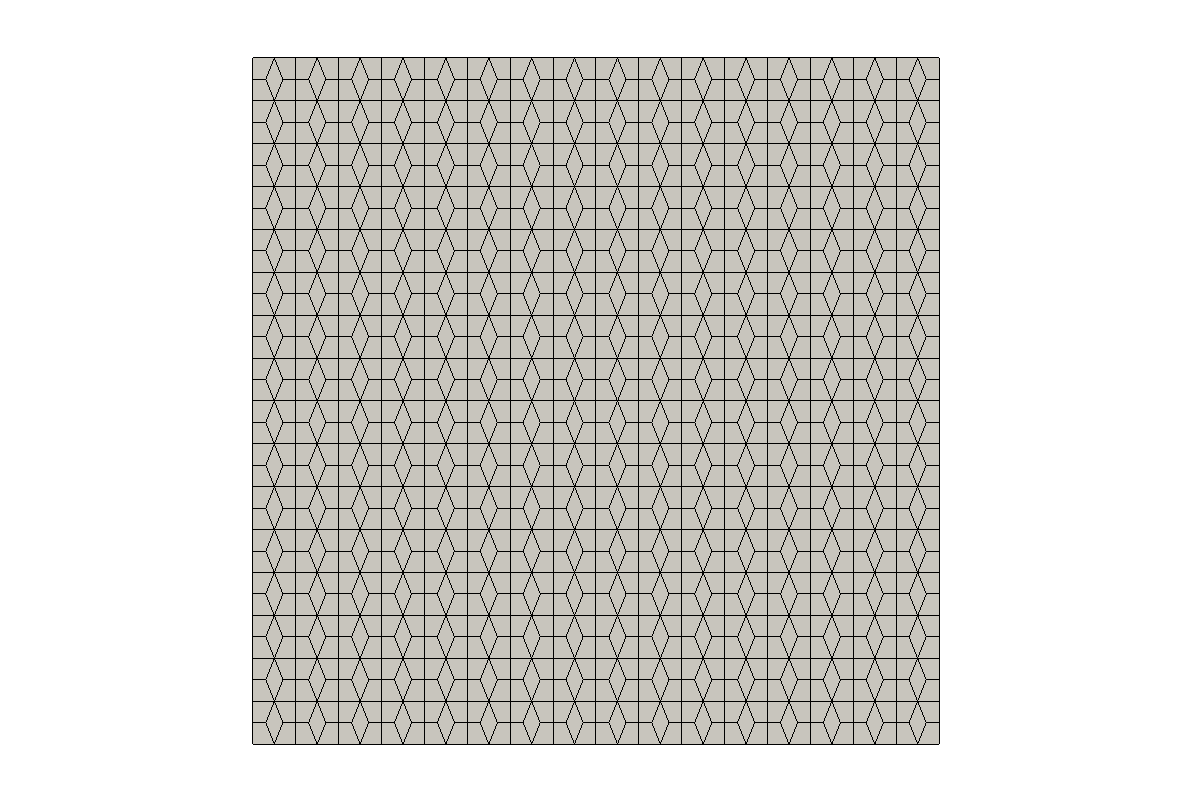
\includegraphics[width=4cm]{python_codes/fieldstone_78/results/mms_dh/16x16/grid0001}
2)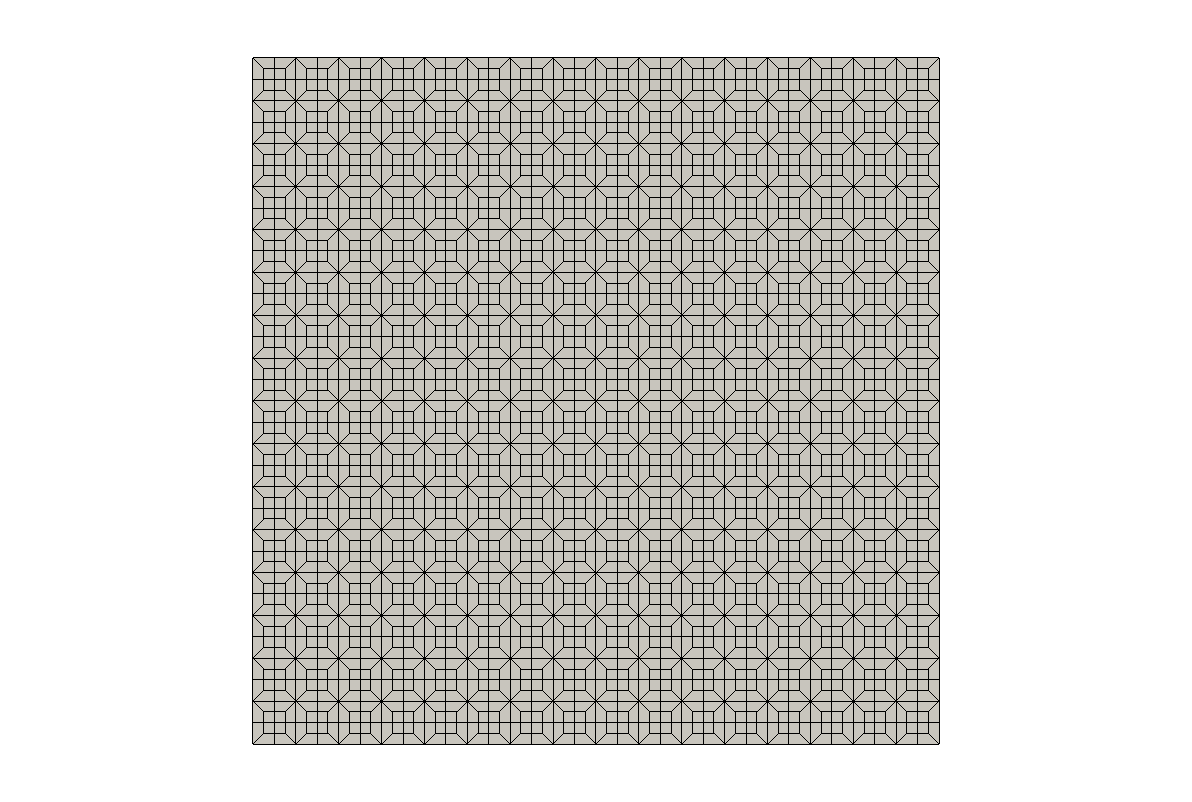
\includegraphics[width=4cm]{python_codes/fieldstone_78/results/mms_dh/16x16/grid0002}
3)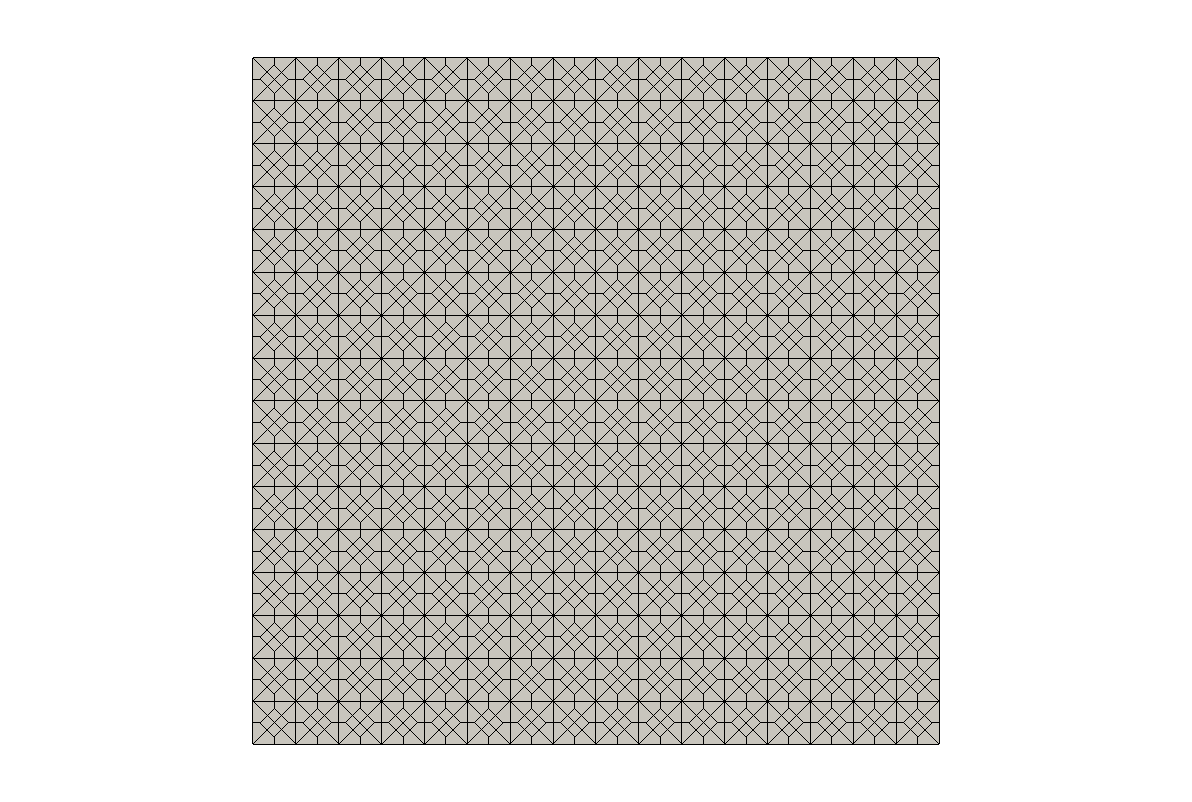
\includegraphics[width=4cm]{python_codes/fieldstone_78/results/mms_dh/16x16/grid0003}\\
4)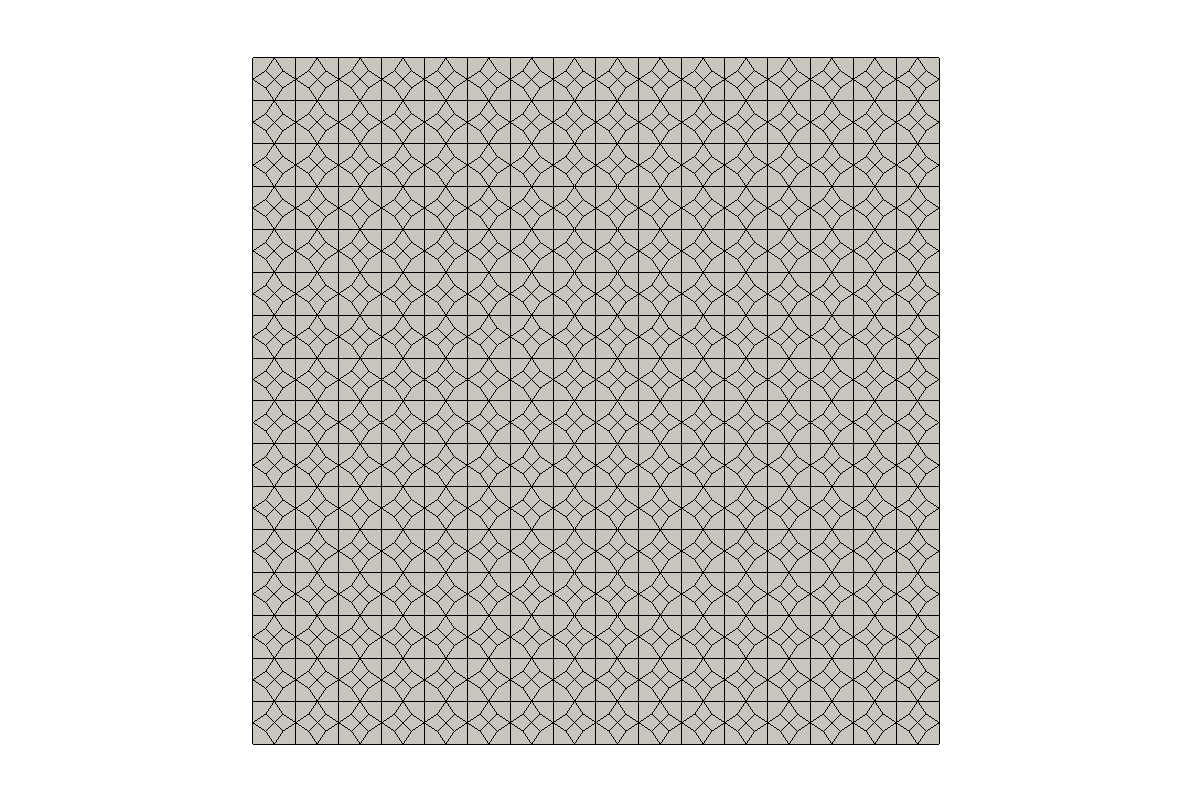
\includegraphics[width=4cm]{python_codes/fieldstone_78/results/mms_dh/16x16/grid0004}
5)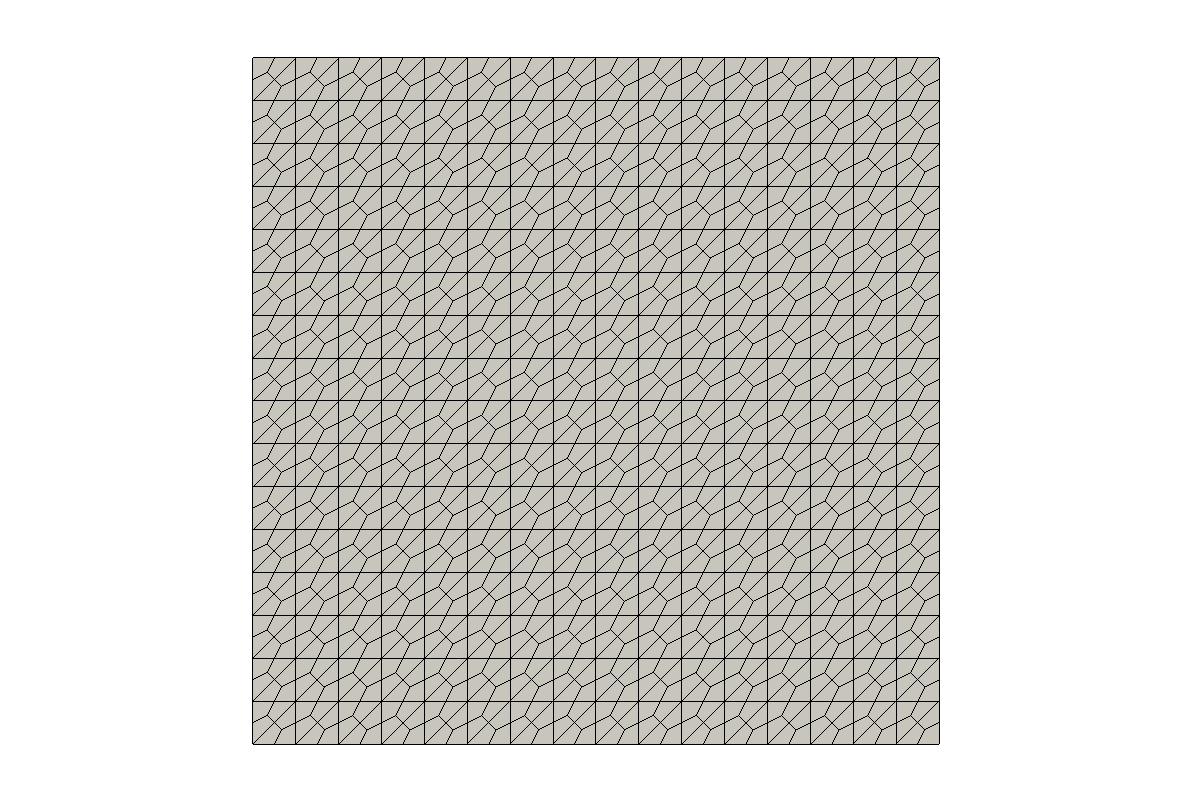
\includegraphics[width=4cm]{python_codes/fieldstone_78/results/mms_dh/16x16/grid0005}
6)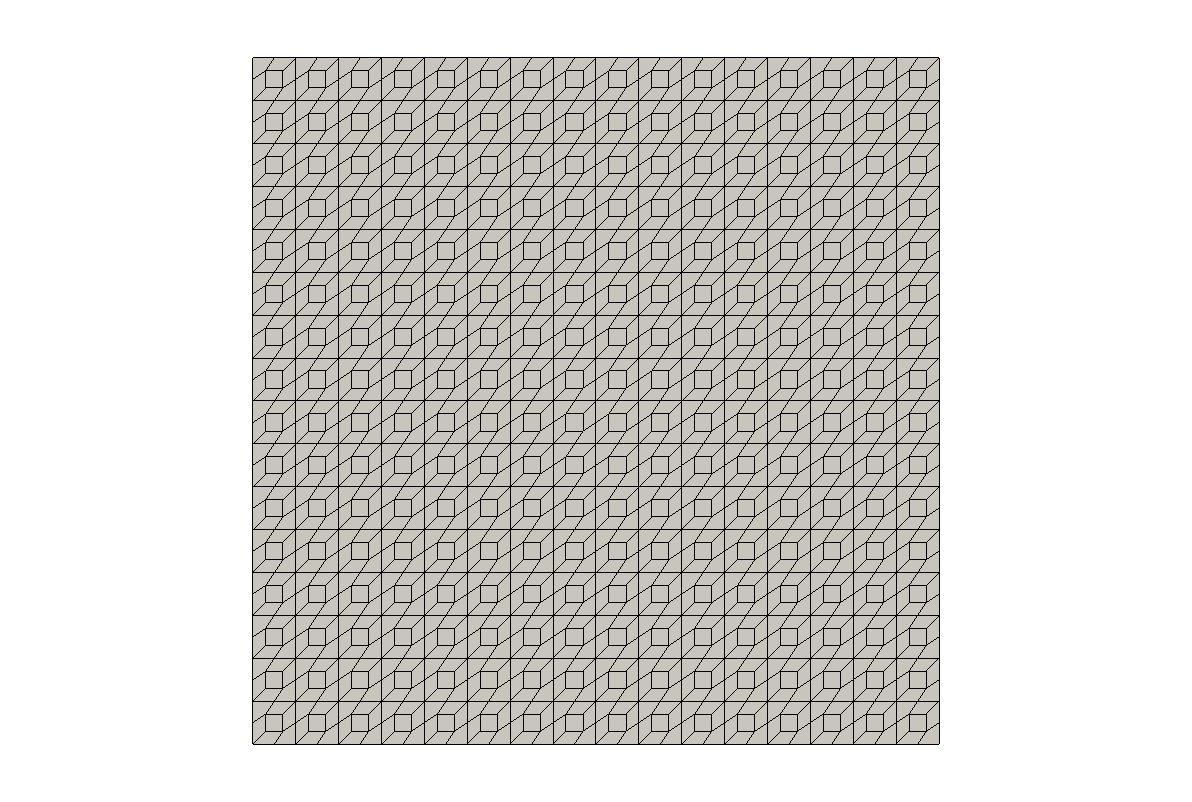
\includegraphics[width=4cm]{python_codes/fieldstone_78/results/mms_dh/16x16/grid0006}
7)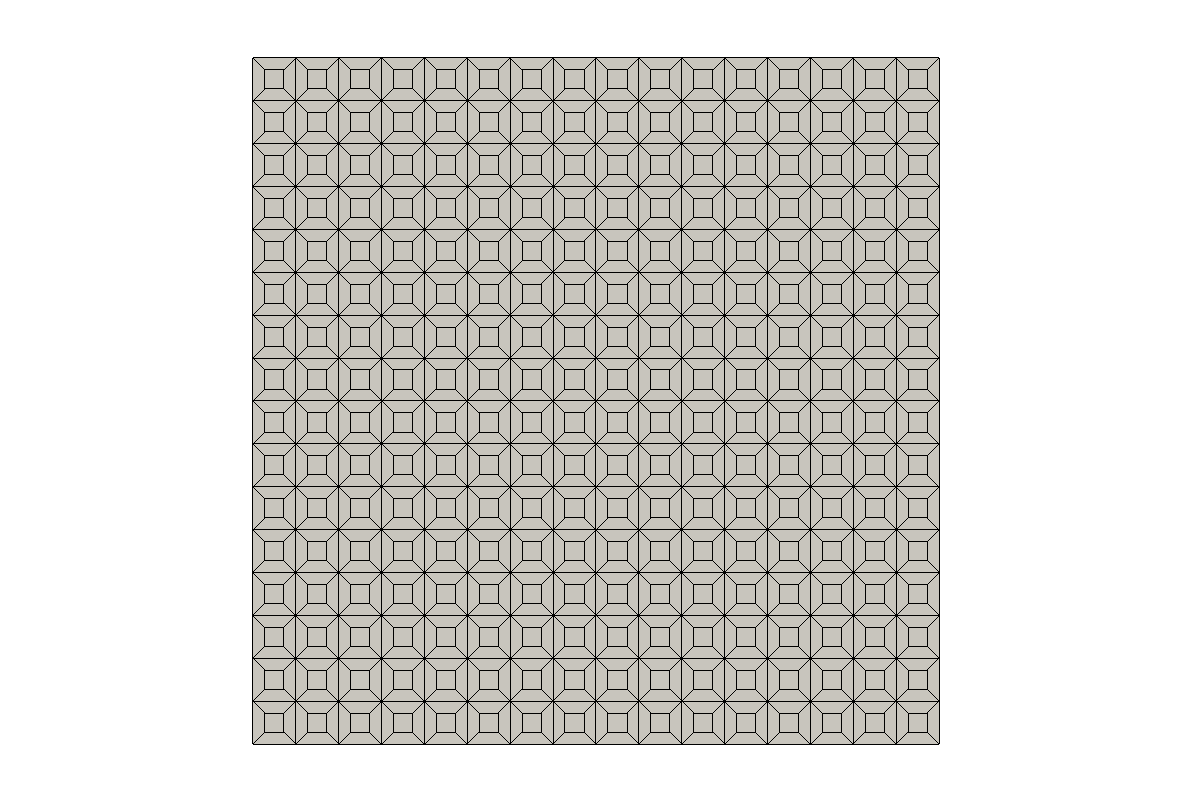
\includegraphics[width=4cm]{python_codes/fieldstone_78/results/mms_dh/16x16/grid0007}\\
{\captionfont 
0: regular structured mesh, 
1: Stenberg (S) \cite{sten84},
2: Le Tallec (LT) \cite{leta81},
3: qizh07 (QZ1) \cite{qizh07} ,
4: qizh07 (QZ2) \cite{qizh07},
5: qizh07 (QZ3) \cite{qizh07},
6: mine (A),
7: mine (B)}
\end{center}


\paragraph{location of nodes inside macro element}.
When possible, we wish that all elements of a macro-element 
have the same area. 
For the Stenberg macro-element, we set $\delta =0.3$.
For the Le Tallex macro-element, we set $\delta=h/\sqrt{12}$.
(dunno where my notes are) 
We also make sure that all elements in QZ1,QZ3,B have same area.
However, there is a problem with QZ2: equi area yields quads with angle =180. 
Likewise macro-element  A cannot be generated with all elements equi-area.



%---------------------------------
\subsection*{Implementation}

There are 14 benchmarks/experiments that are currently implemented in the code:
\begin{enumerate}
\item Donea \& Huerta (MS) %1
\item block in the middle %2
\item sphere in the middle %3
\item aquarium %4
\item SolKz (MS) %5
\item regularised lid driven cavity %6
\item cavity (MS) %7
\item sinking block %8
\item Dohrmann \& Bochev (MS) \cite{dobo04} %9
\item flow around square cylinder % 10
\item flow over cavity % 11
\item flow over obstacle %12
\item SolCx (MS) %13
\item SolVi (MS) %14
\end{enumerate}
where MS stands for `manufactured solution'.

All experiments take place in the unit square expect experiment 8.

All experiments are isoviscous expect 3,5,8,13,14.
Note that the viscosity is evaluated in the middle of each element, not 
at the quadrature points. This can/will have an effect on non-isoviscous models.

\newpage
The meshes are created by importing the corresponding files:
\begin{lstlisting} 
import regular
import macro_S
import macro_LT
import macro_QZ1 
import macro_QZ2
import macro_QZ3
import macro_A
import macro_B
\end{lstlisting} 
Inside each of these files a function called {\sl mesher} is defined: 
\begin{lstlisting} 
def mesher(Lx,Ly,nelx,nely,nel,NV,mV):
\end{lstlisting} 
The arguments are the domain size $L_x$ and $L_y$, the number of macroelements
in each direction $nelx$ and $nely$, the precomputed total number of $Q_1\times P_0$ 
elements $nel$ and nodes $NV$ and the number of nodes per element $m_\upnu$.  

Pressure normalisation is achieved by enforcing after the solve:
\[
\int_\Omega p dV = \sum_e A_e p_e = 0
\]
where $A_e$ is the area of element $e$.

In what follows $p$ is the 'raw' pressure field (after normalisation)
while $q$ denotes its projection onto the nodes by means of corner-to-node average.
More specifically $q_1$ is the pressure average at the node, 
while $q_2$  is the element area weighed average.

Define errors and mesh size which is taken to be $h = \sqrt{L_xL_y/nel}$. 


\newpage
%-----------------------------------------------------------------
\subsection*{Experiment 1: Donea \& Huerta (MS)}

We start with the Donea \& Huerta manufactured solution (see Section~\ref{MMM-mms1}) and 
proceed to compute the velocity and pressure error convergence as a function of the 
average element size.
we see that the errors converge as expected, quadratically for the velocity and linearly for the pressure.
Rather interestingly the projection of the pressure onto the nodes has a convergence rate 
higher than the raw elemental pressure. As predicted in Qin \& Zhang, the Stenberg macro-element 
yields the best results, followed by the Le Tallec and then the one they propose (this conclusion 
is logically supported by looking at root mean square velocity measurements). 
Finally, the presence of the checkerboard for the regular structure mesh case
makes it painfully clear that it is the worst mesh topology 
and the pressure error does not converge.  

\begin{center}
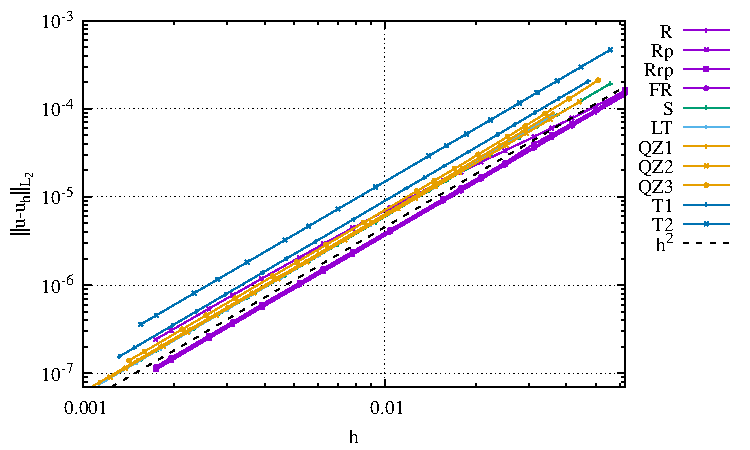
\includegraphics[width=5cm]{python_codes/fieldstone_78/results/errors_u_exp1.pdf}
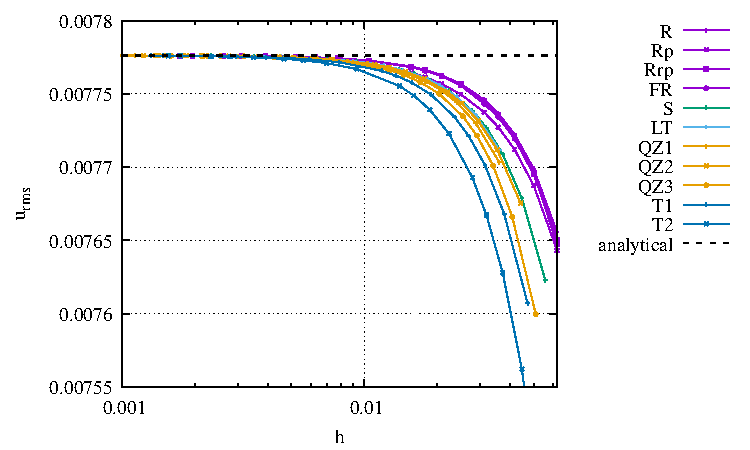
\includegraphics[width=5cm]{python_codes/fieldstone_78/results/vrms_exp1.pdf} \\
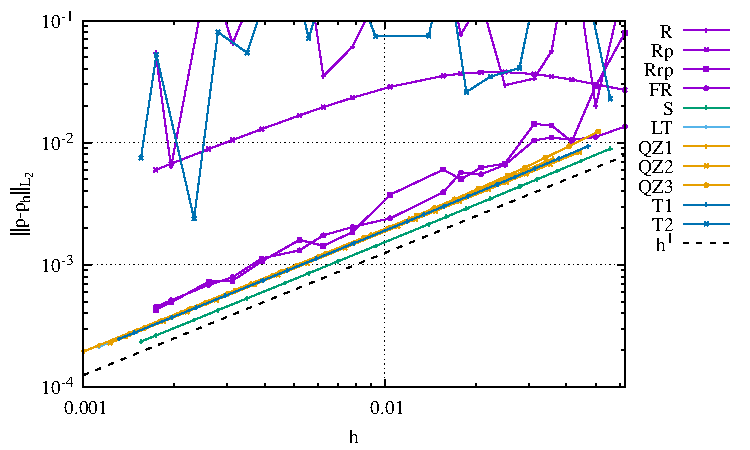
\includegraphics[width=5cm]{python_codes/fieldstone_78/results/errors_p_exp1.pdf}
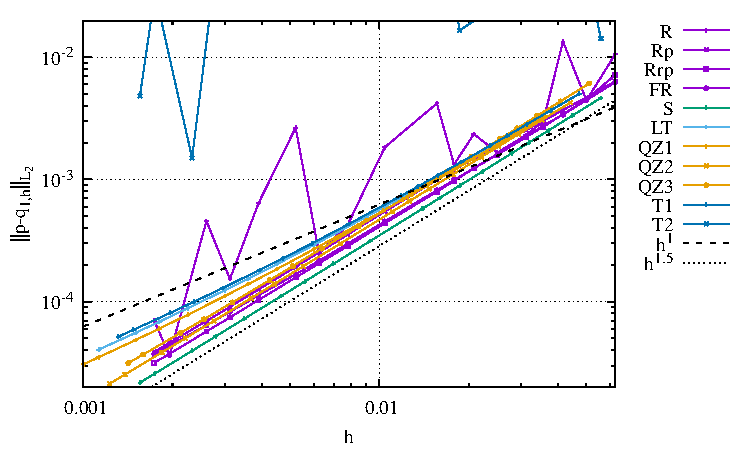
\includegraphics[width=5cm]{python_codes/fieldstone_78/results/errors_q1_exp1.pdf}
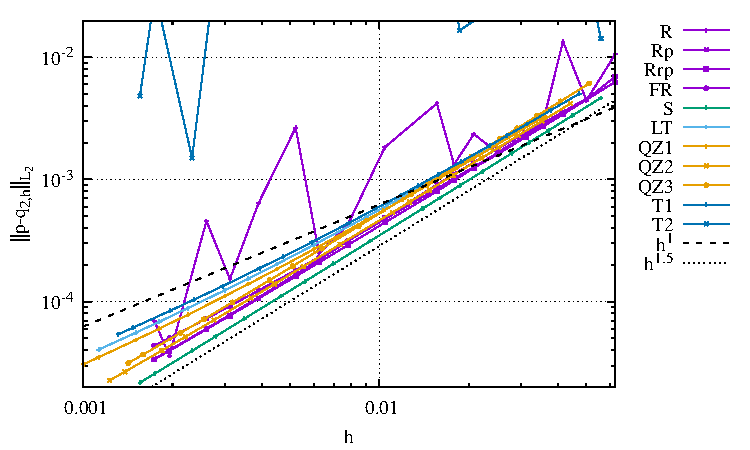
\includegraphics[width=5cm]{python_codes/fieldstone_78/results/errors_q2_exp1.pdf}\\
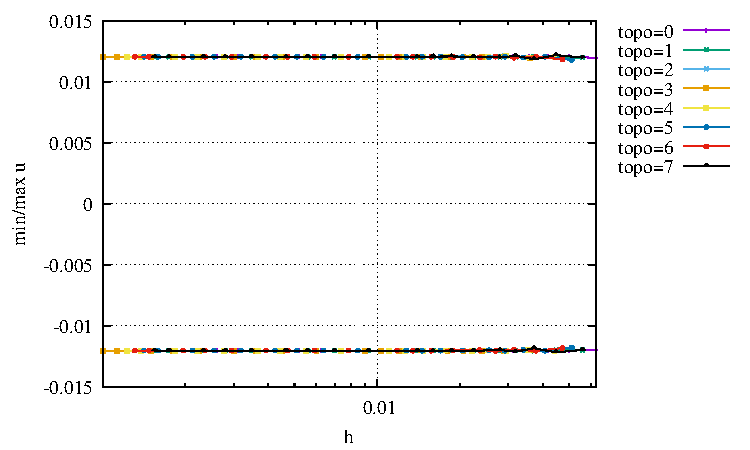
\includegraphics[width=5cm]{python_codes/fieldstone_78/results/stats_u_exp1.pdf}
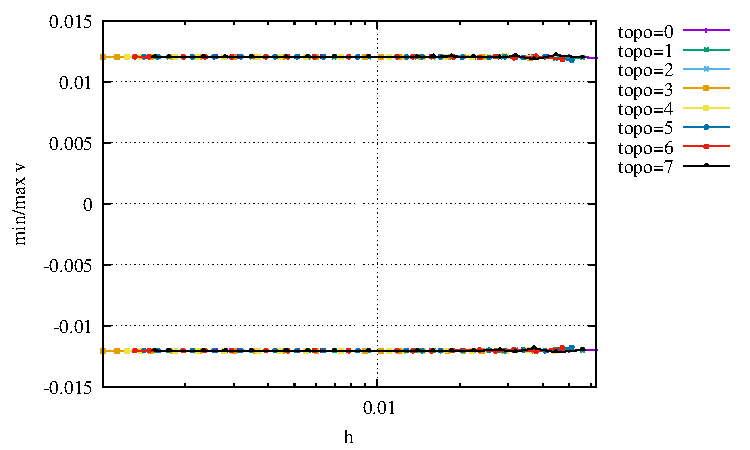
\includegraphics[width=5cm]{python_codes/fieldstone_78/results/stats_v_exp1.pdf}\\
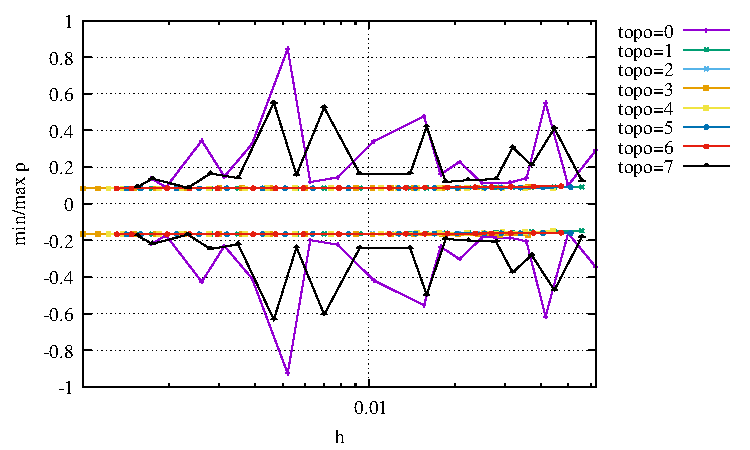
\includegraphics[width=5cm]{python_codes/fieldstone_78/results/stats_p_exp1.pdf}
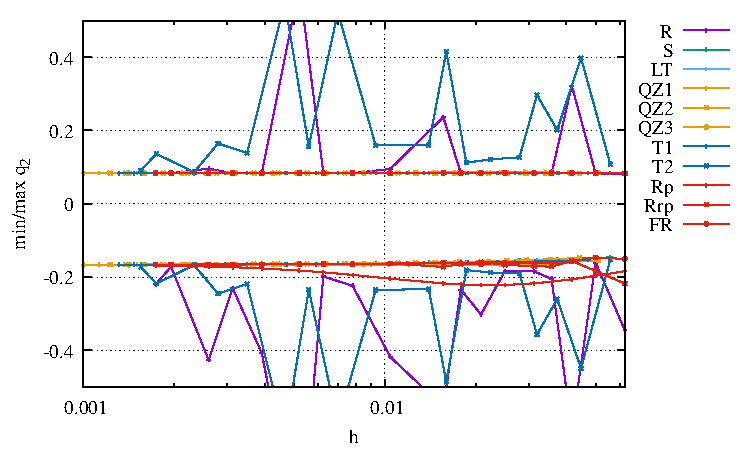
\includegraphics[width=5cm]{python_codes/fieldstone_78/results/stats_q1_exp1.pdf}
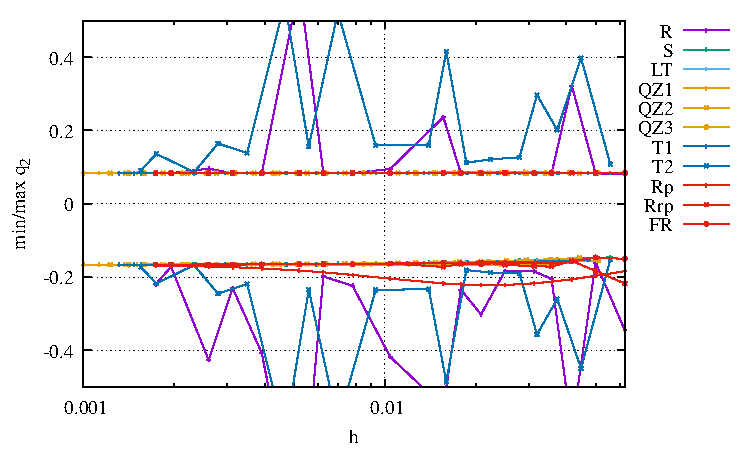
\includegraphics[width=5cm]{python_codes/fieldstone_78/results/stats_q2_exp1.pdf}
\end{center}

On the following figures the pressure is plotted against the analytical solution and 
we see that there is no checkerboarding occurring:
Rather interestingly the pressure error is the largest next to the boundaries.

\begin{center}
0)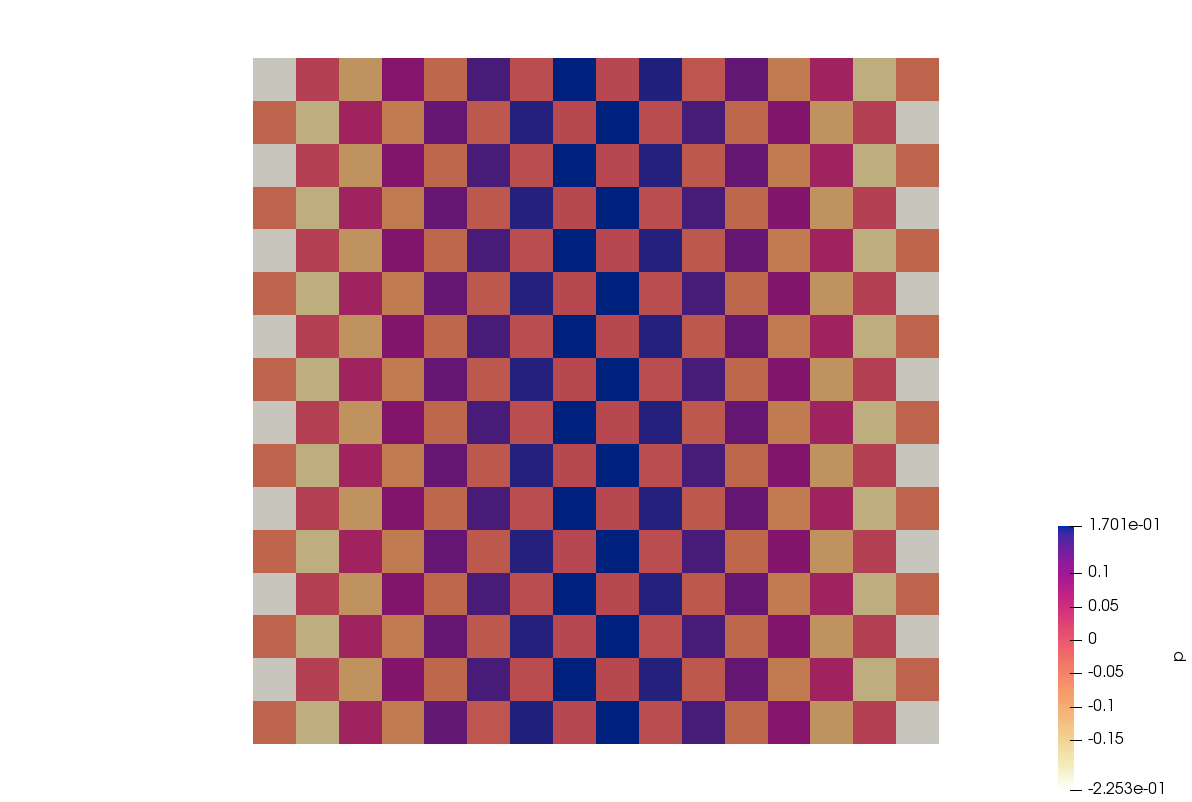
\includegraphics[width=4cm]{python_codes/fieldstone_78/results/mms_dh/16x16/p0}
1)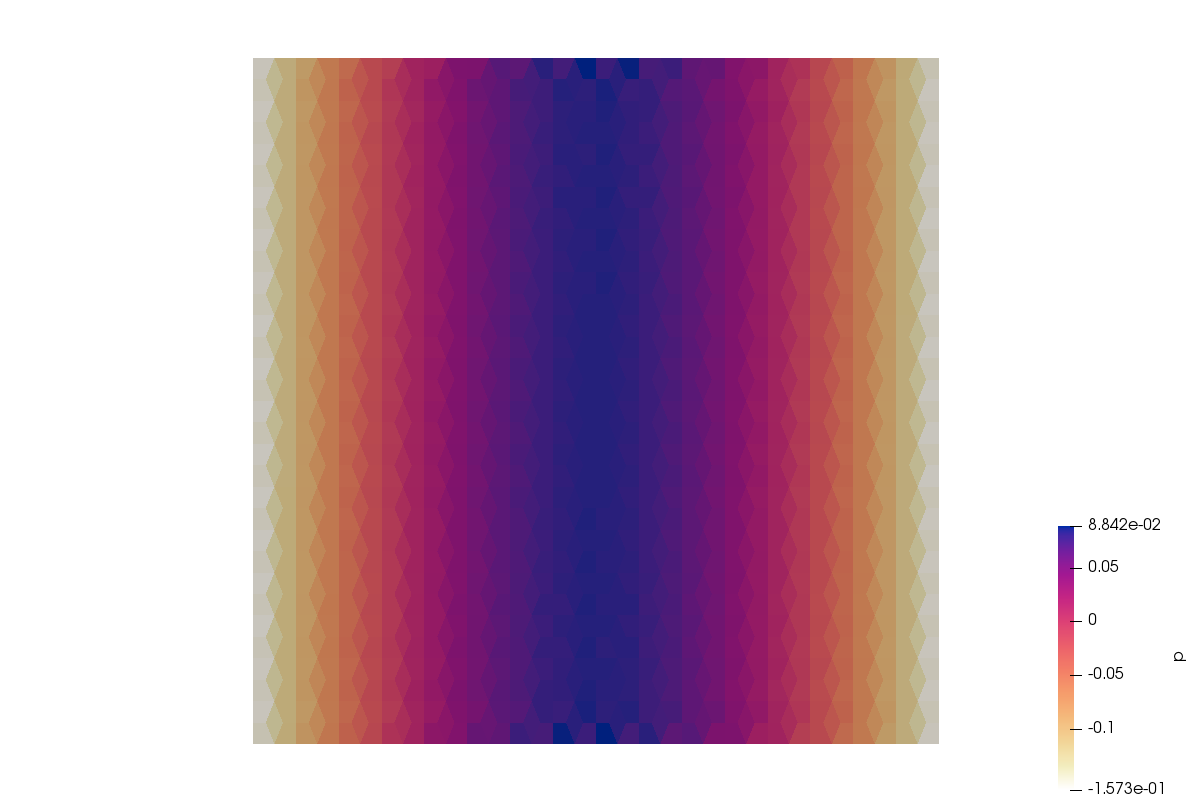
\includegraphics[width=4cm]{python_codes/fieldstone_78/results/mms_dh/16x16/p1}
2)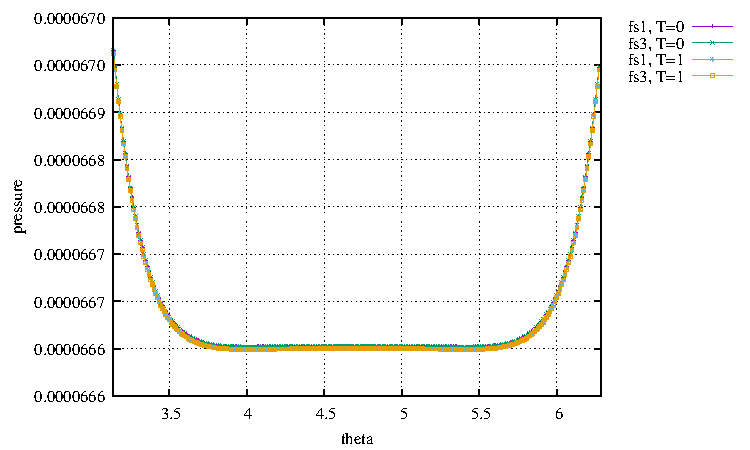
\includegraphics[width=4cm]{python_codes/fieldstone_78/results/mms_dh/16x16/p2}
3)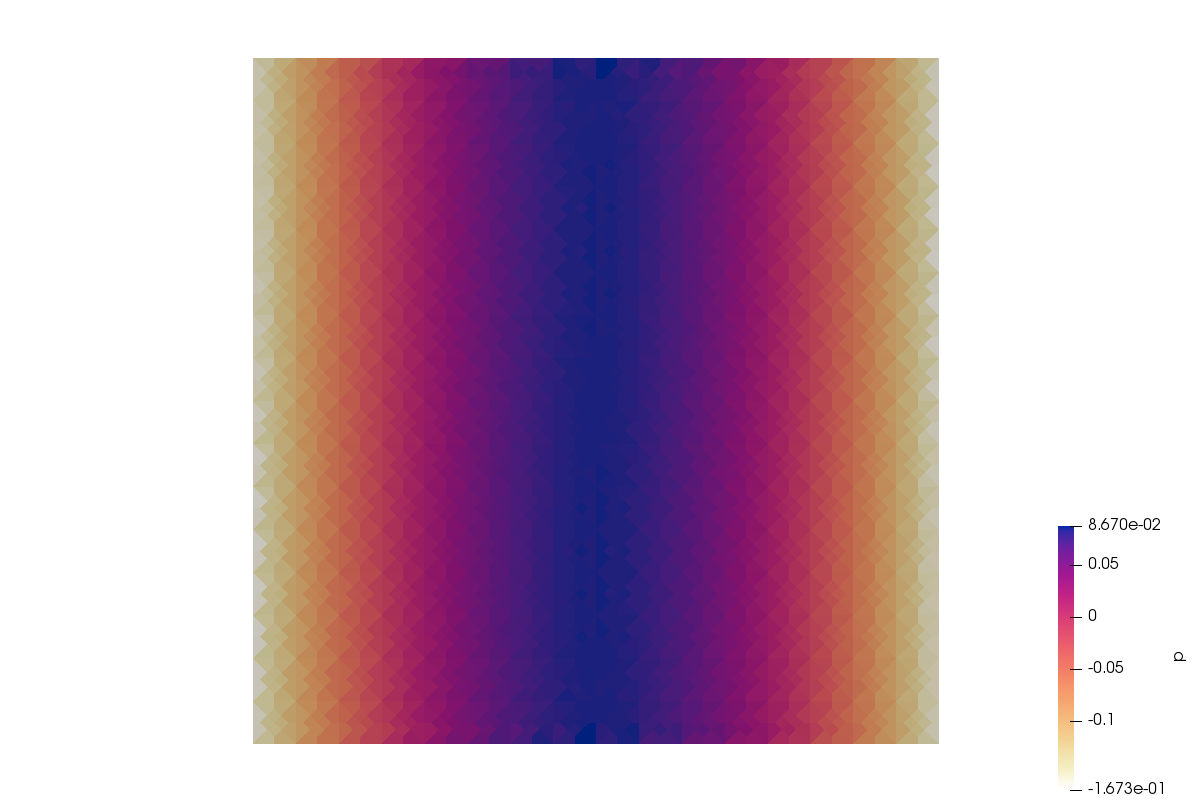
\includegraphics[width=4cm]{python_codes/fieldstone_78/results/mms_dh/16x16/p3}\\
4)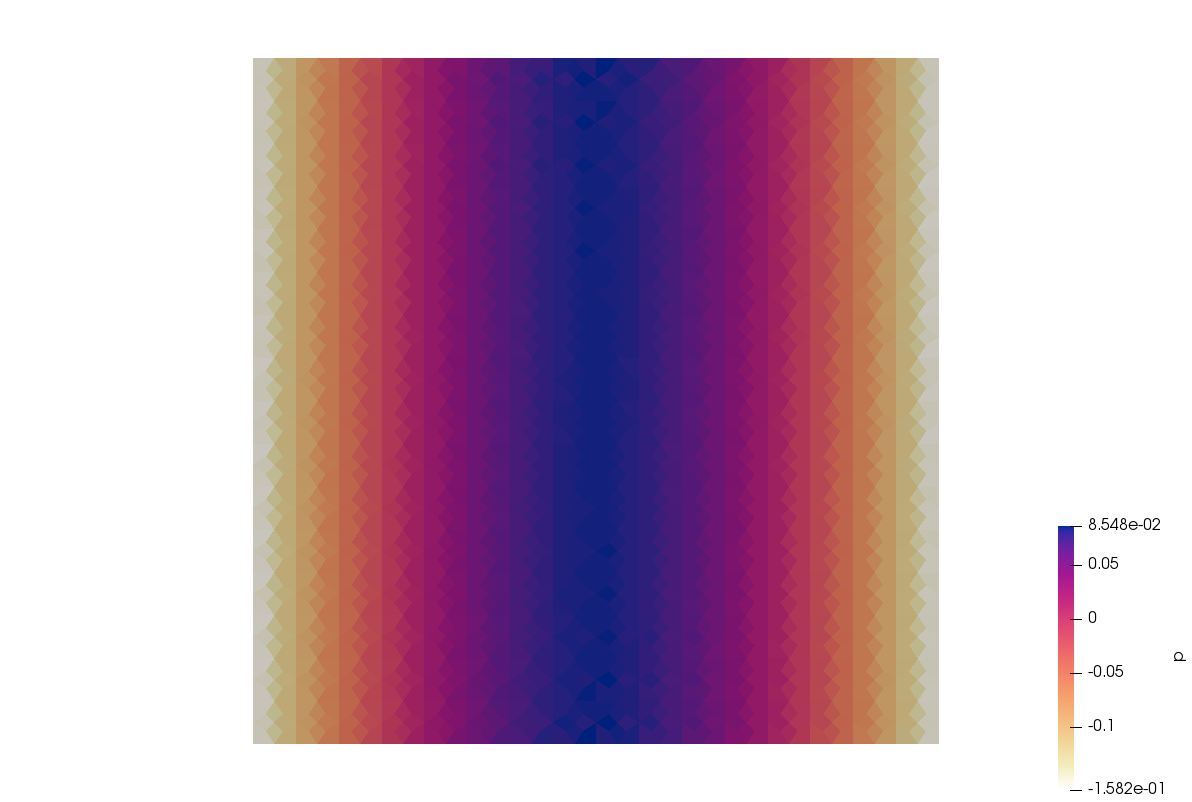
\includegraphics[width=4cm]{python_codes/fieldstone_78/results/mms_dh/16x16/p4}
5)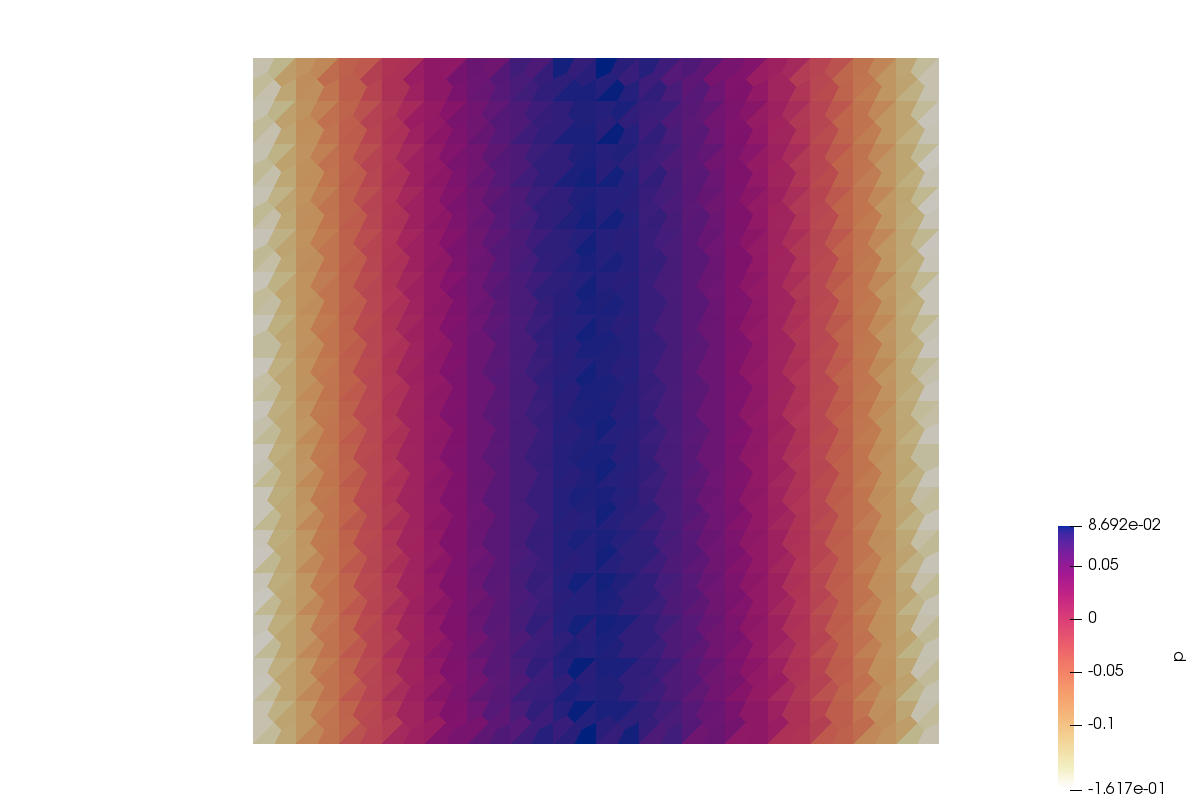
\includegraphics[width=4cm]{python_codes/fieldstone_78/results/mms_dh/16x16/p5}
6)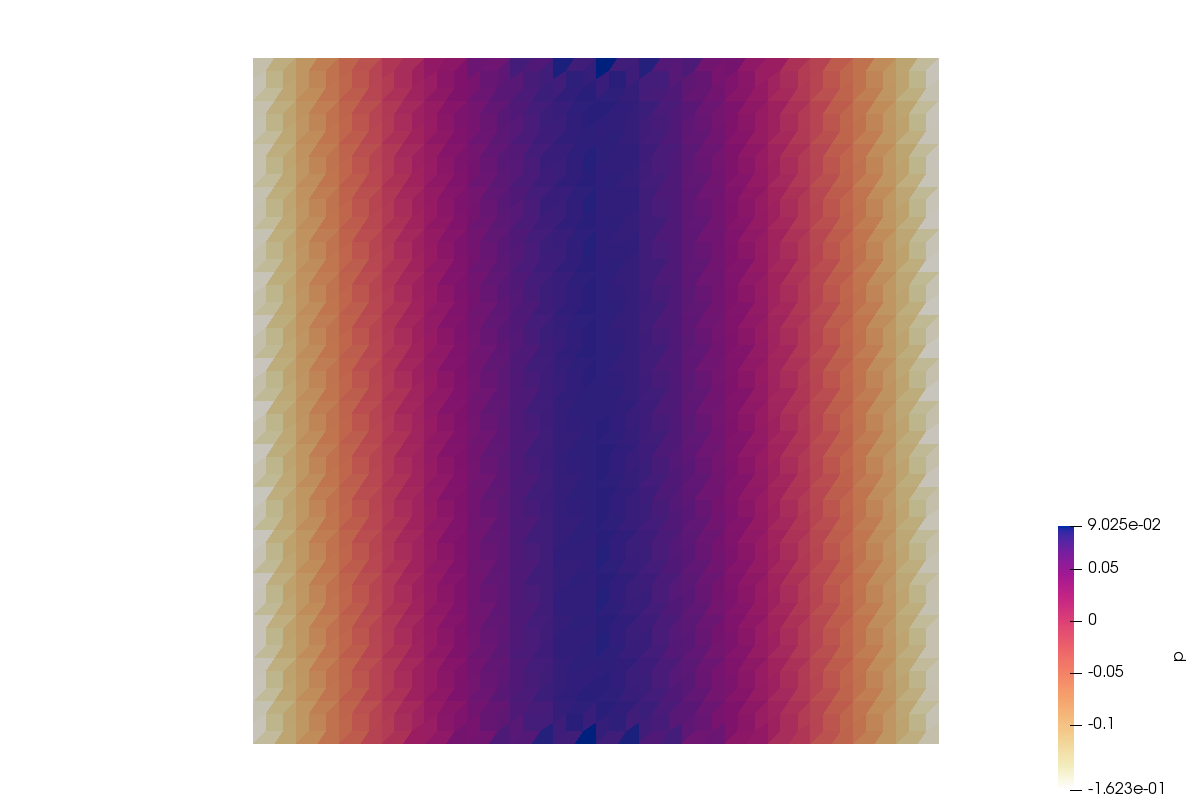
\includegraphics[width=4cm]{python_codes/fieldstone_78/results/mms_dh/16x16/p6}
7)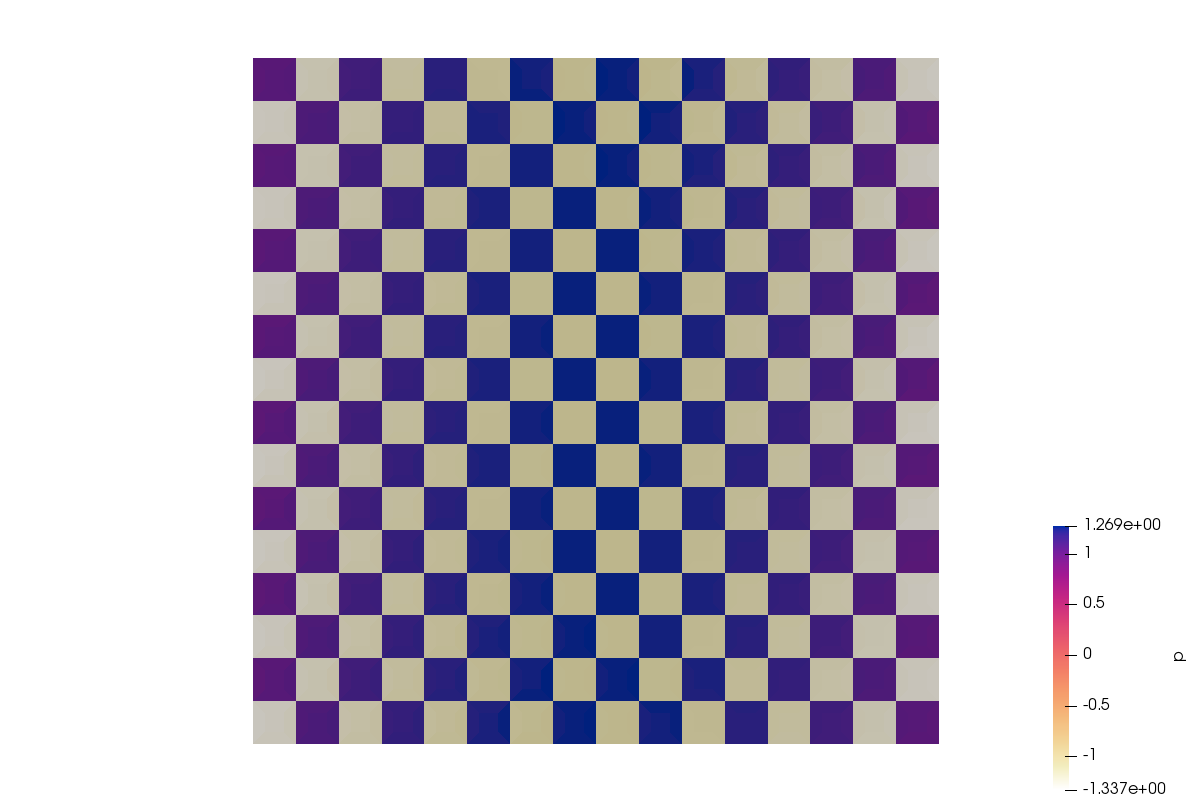
\includegraphics[width=4cm]{python_codes/fieldstone_78/results/mms_dh/16x16/p7}\\
{\captionfont Meshes  made of 16x16 (macro-)elements.} 
\end{center}


\newpage
%-------------------------------------------------------------
\subsection*{Experiment 2: Dimensionless sinking square (EXP)}

The block has size $0.25\times 0.25$, centered in the domain. No-slip boundary conditions are imposed on all 
sides. The buoyancy force $\rho g_y$ is -1 in the block and zero elsewhere. Viscosity is constant and 
equal to 1 everywhere. 

\begin{center}
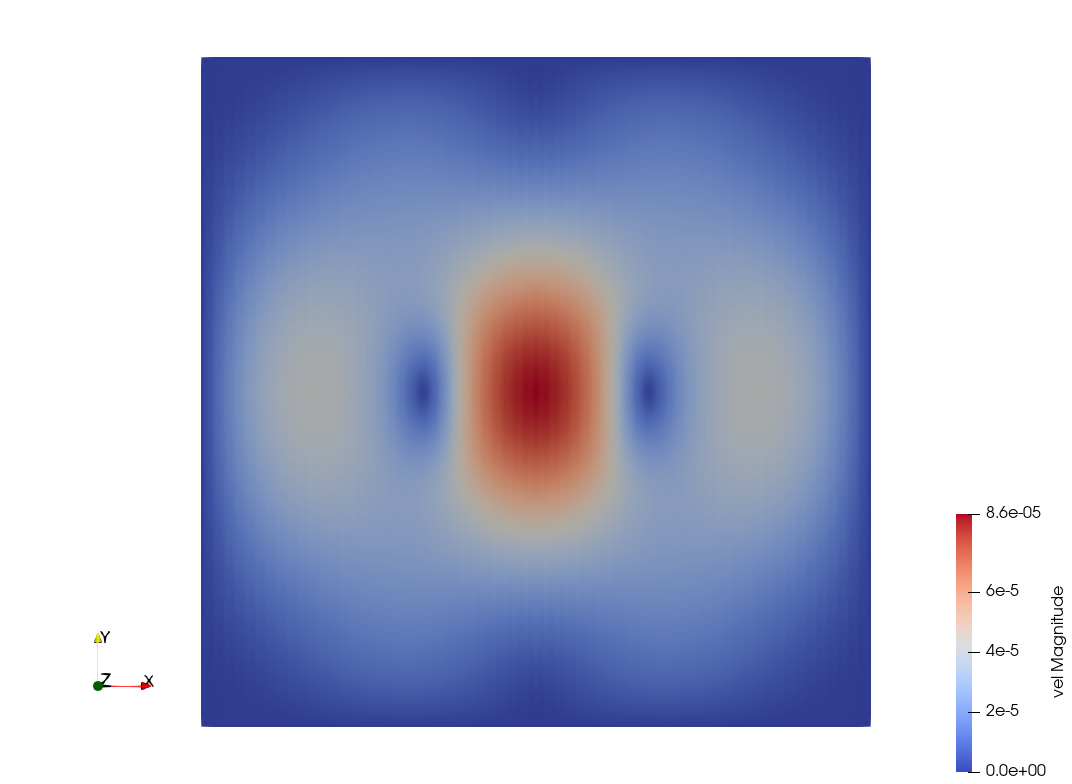
\includegraphics[width=5cm]{python_codes/fieldstone_78/results/exp02/vel}
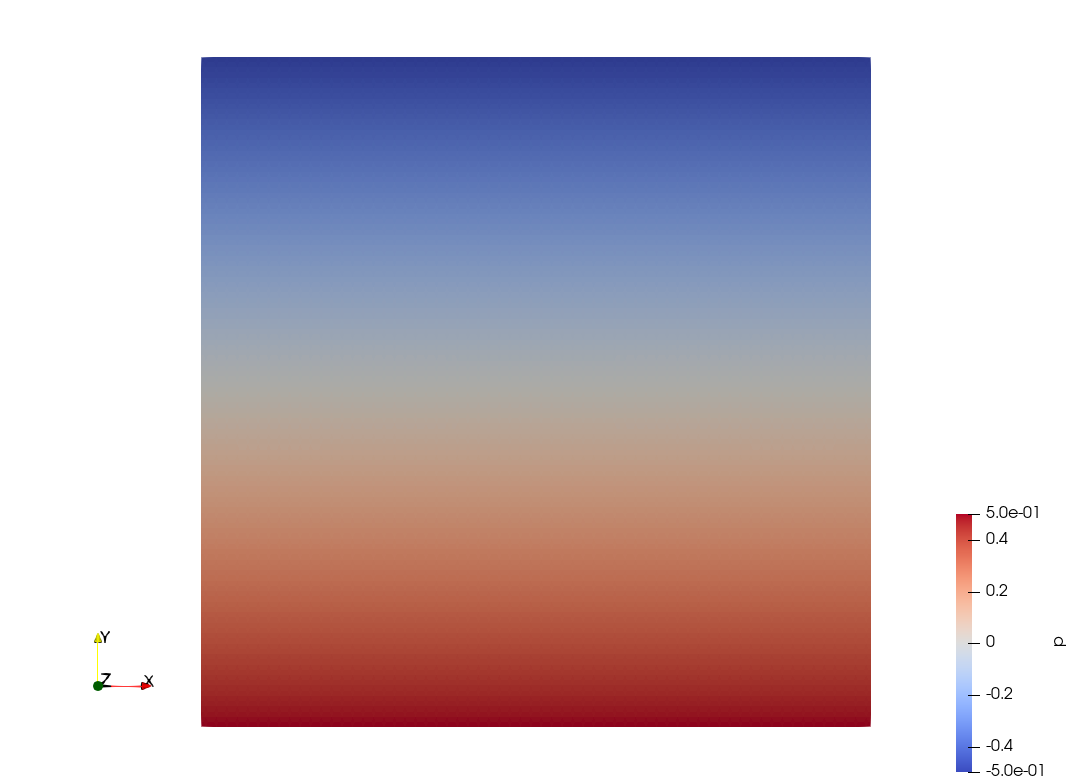
\includegraphics[width=5cm]{python_codes/fieldstone_78/results/exp02/p}
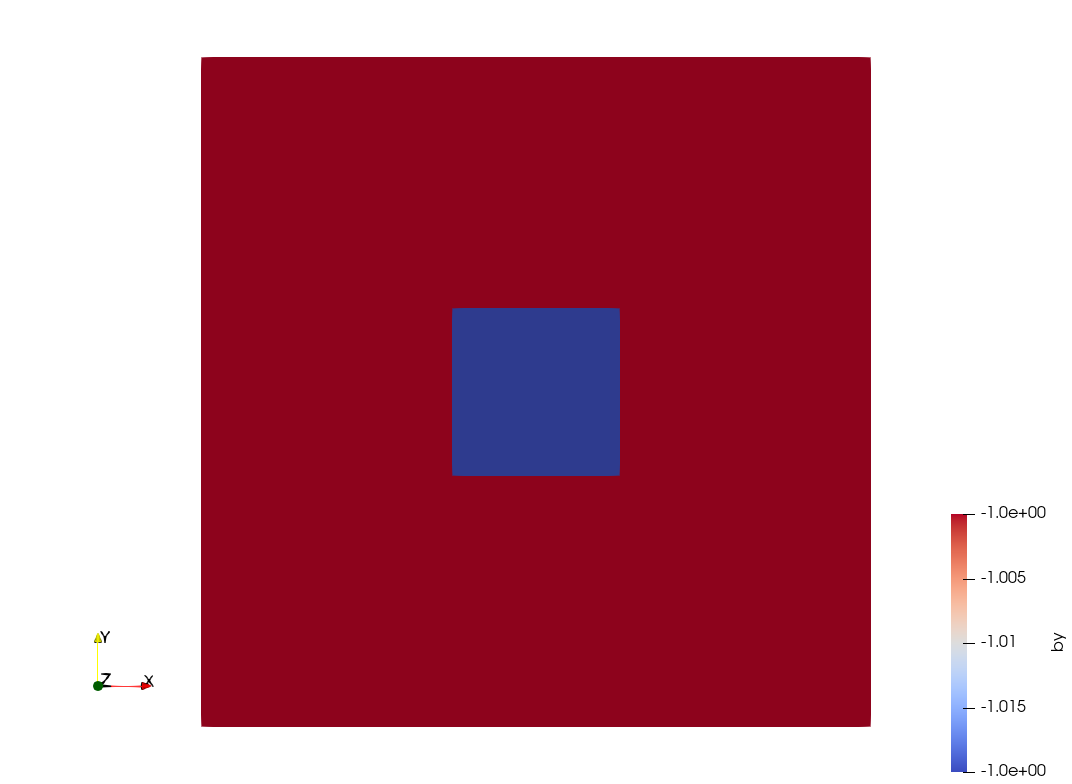
\includegraphics[width=5cm]{python_codes/fieldstone_78/results/exp02/by}\\
{\captionfont Stenberg, 64x64.}
\end{center}

\begin{center}
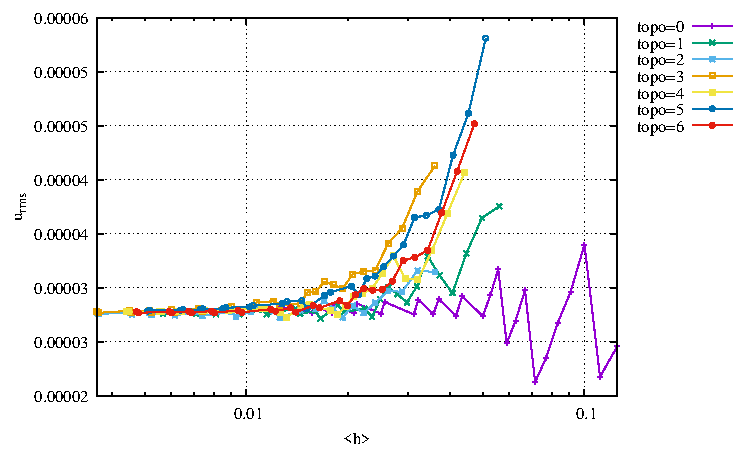
\includegraphics[width=5cm]{python_codes/fieldstone_78/results/vrms_exp2.pdf} 
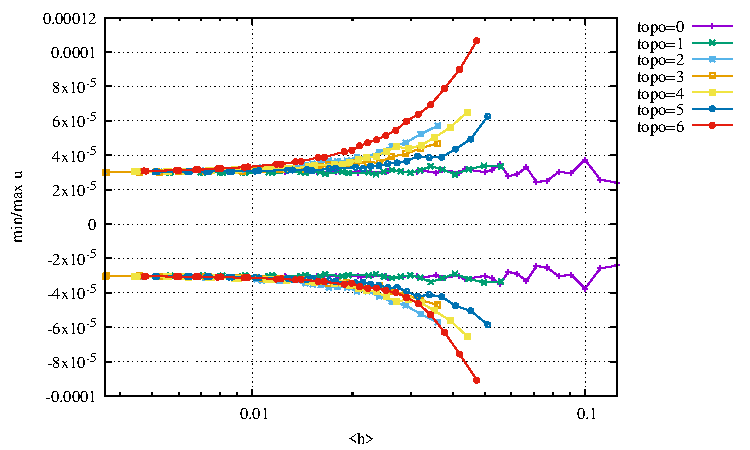
\includegraphics[width=5cm]{python_codes/fieldstone_78/results/stats_u_exp2.pdf}
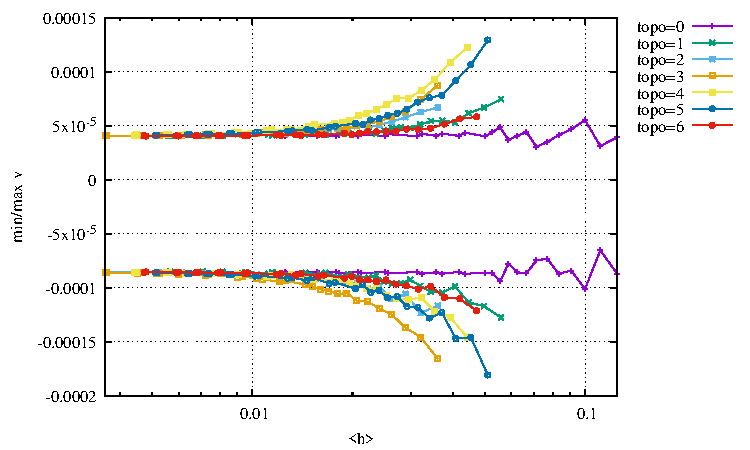
\includegraphics[width=5cm]{python_codes/fieldstone_78/results/stats_v_exp2.pdf}\\
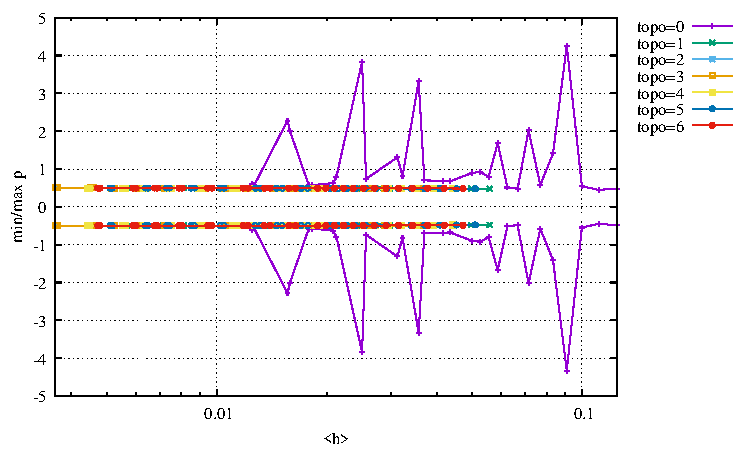
\includegraphics[width=5cm]{python_codes/fieldstone_78/results/stats_p_exp2.pdf}
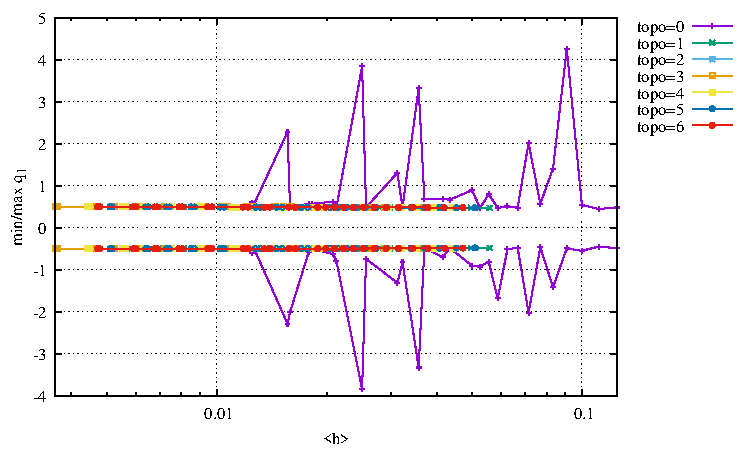
\includegraphics[width=5cm]{python_codes/fieldstone_78/results/stats_q1_exp2.pdf}
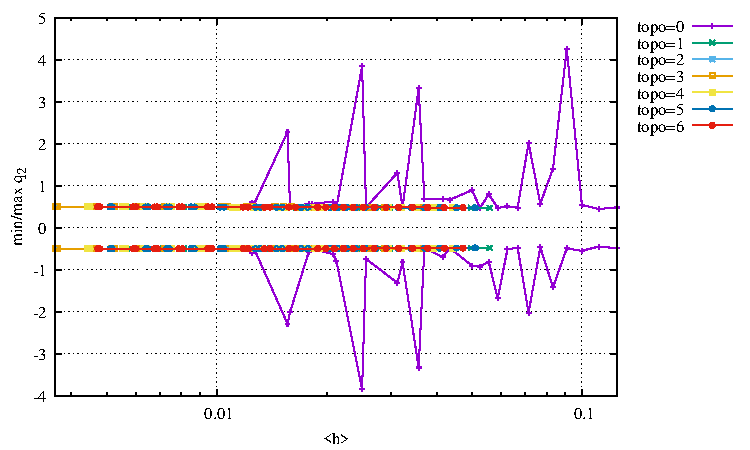
\includegraphics[width=5cm]{python_codes/fieldstone_78/results/stats_q2_exp2.pdf}
\end{center}


\begin{center}
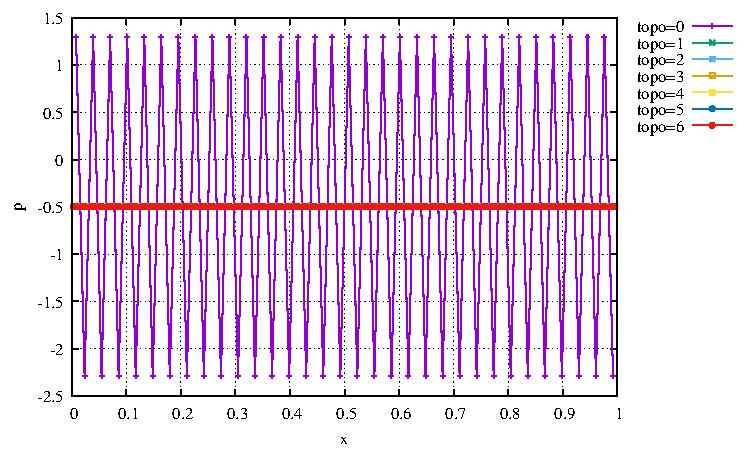
\includegraphics[width=5cm]{python_codes/fieldstone_78/results/pressure_top_exp2.pdf}
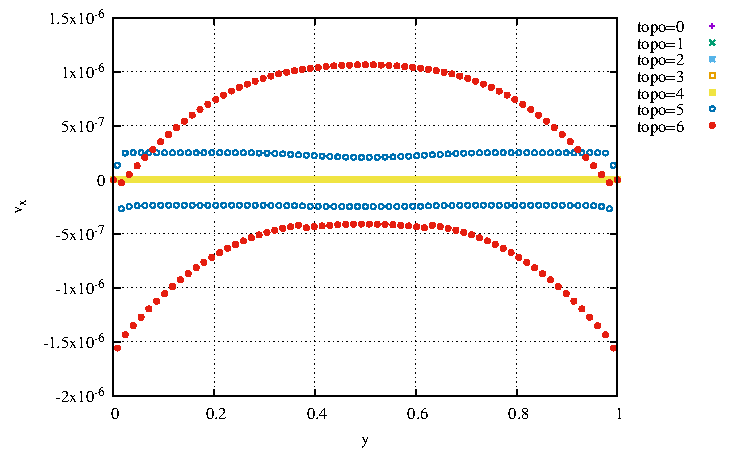
\includegraphics[width=5cm]{python_codes/fieldstone_78/results/vx_profile_exp2.pdf}
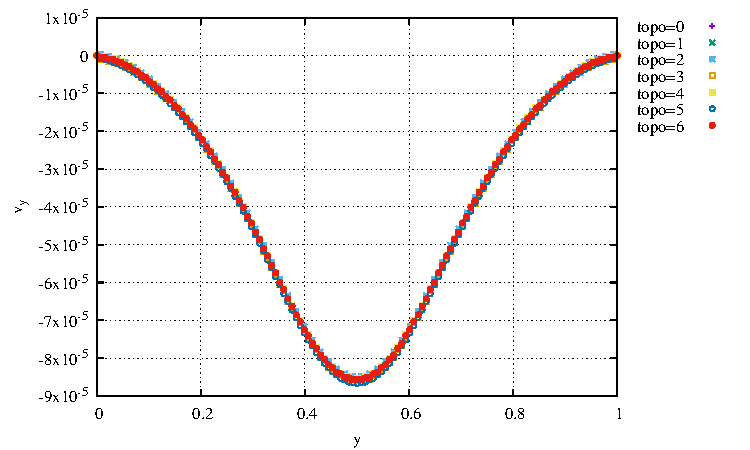
\includegraphics[width=5cm]{python_codes/fieldstone_78/results/vy_profile_exp2.pdf}\\
{\captionfont Left: Pressure at the surface; Middle, Right: velocity on vertical line in the middle.}
\end{center}




\newpage
%-------------------------------------------------------------
\subsection*{Experiment 3: Dimensionless sinking sphere (EXP)}

This is the same experiment as above, except for the geometry of the object 
which is now a sphere of radius 0.125 so that the interface between both fluids 
is never aligned with the mesh/element edges. The sphere has density is 1 while the surrounding is 0.
Its viscosity is $10^4$ while the surrounding is 1.

\begin{center}
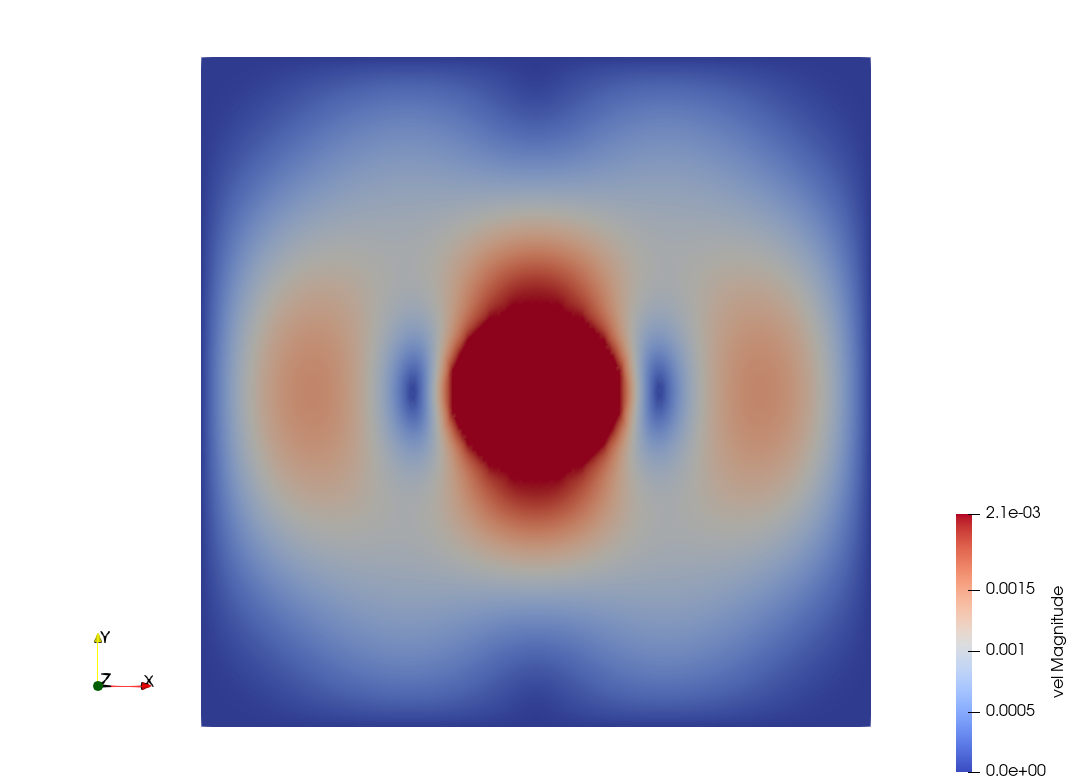
\includegraphics[width=4cm]{python_codes/fieldstone_78/results/exp03/vel}
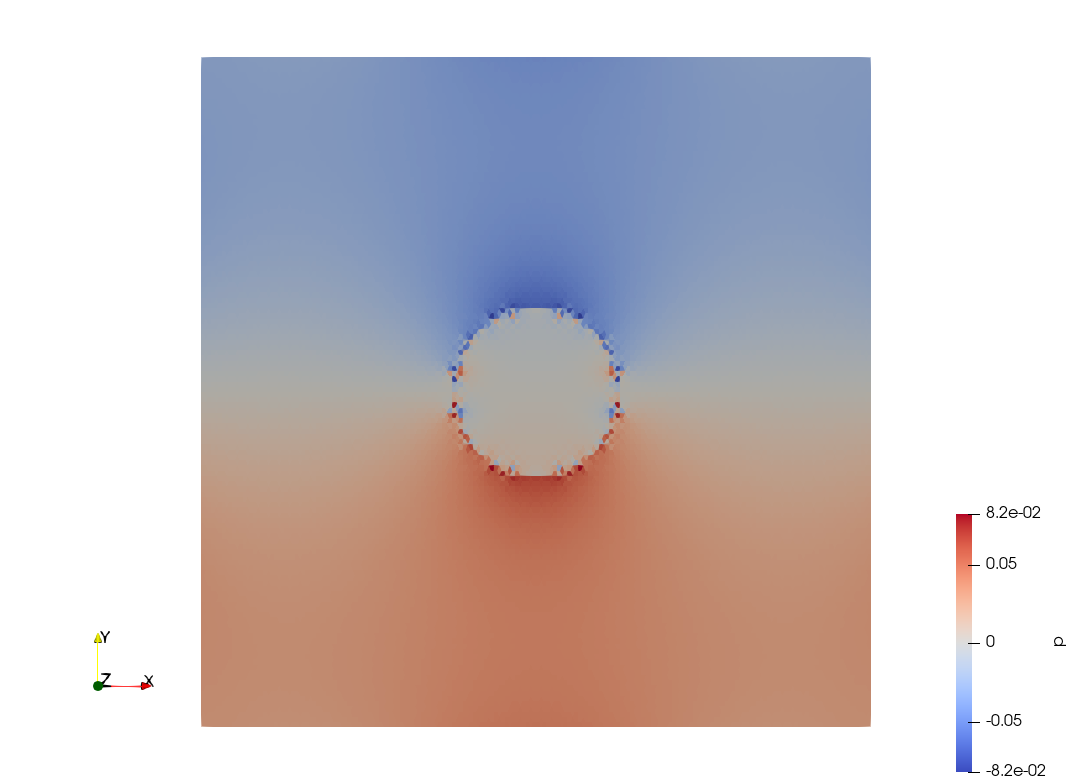
\includegraphics[width=4cm]{python_codes/fieldstone_78/results/exp03/p}
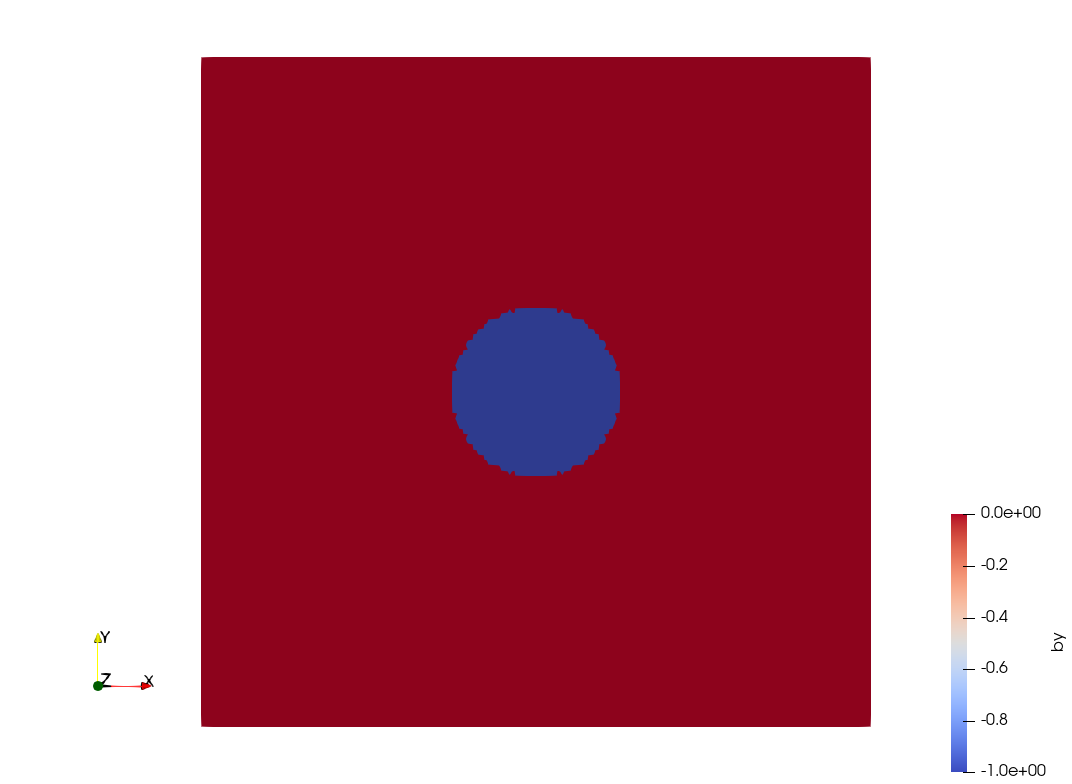
\includegraphics[width=4cm]{python_codes/fieldstone_78/results/exp03/by}
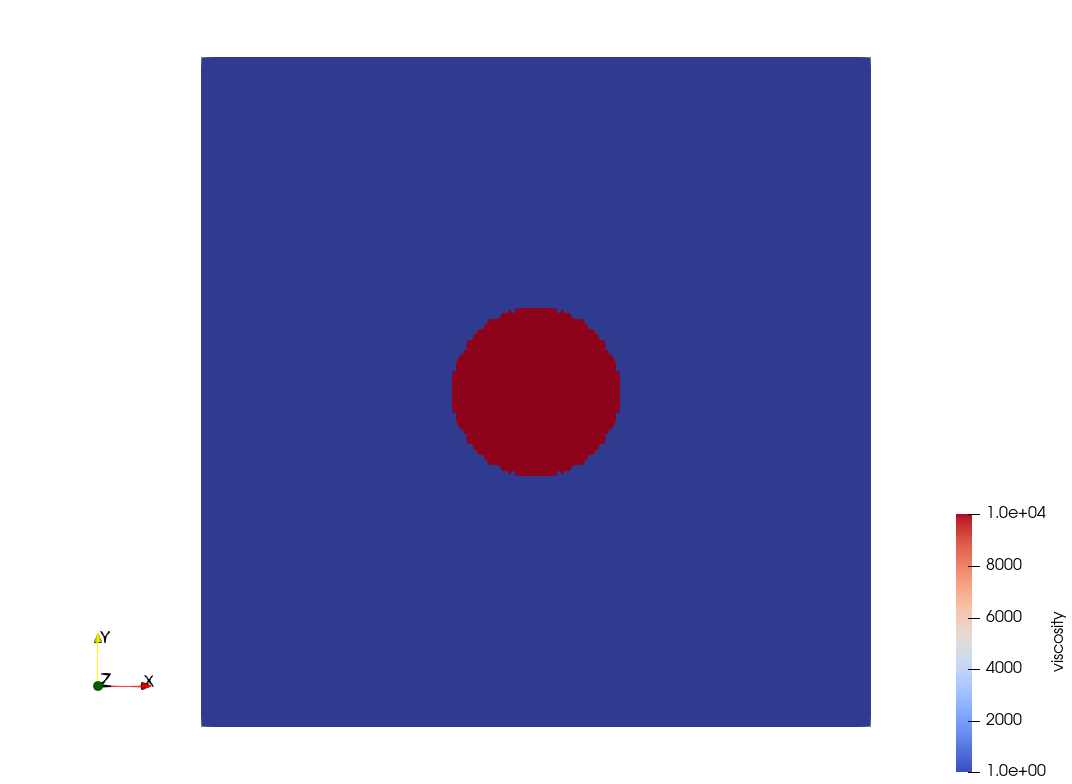
\includegraphics[width=4cm]{python_codes/fieldstone_78/results/exp03/viscosity}\\
{\captionfont Stenberg, 64x64.}
\end{center}

\begin{center}
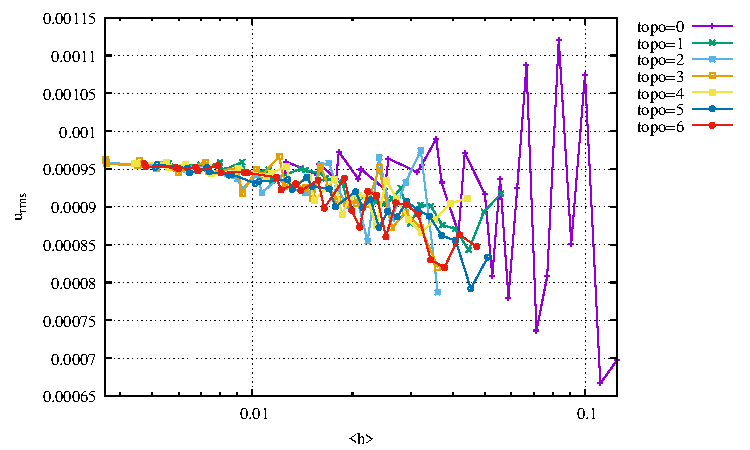
\includegraphics[width=5cm]{python_codes/fieldstone_78/results/vrms_exp3.pdf} 
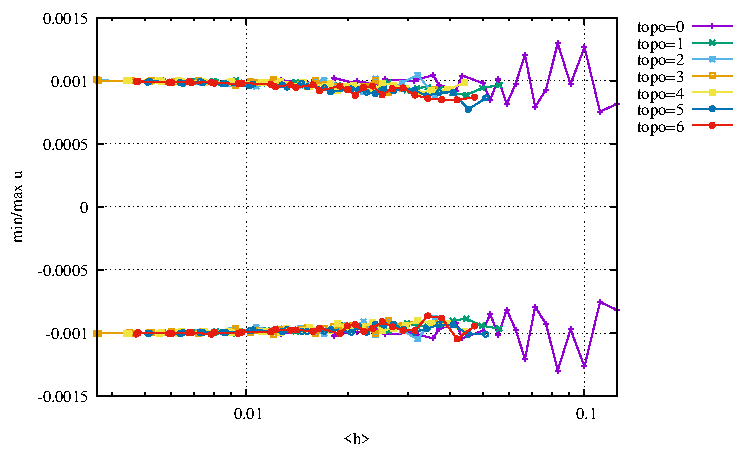
\includegraphics[width=5cm]{python_codes/fieldstone_78/results/stats_u_exp3.pdf}
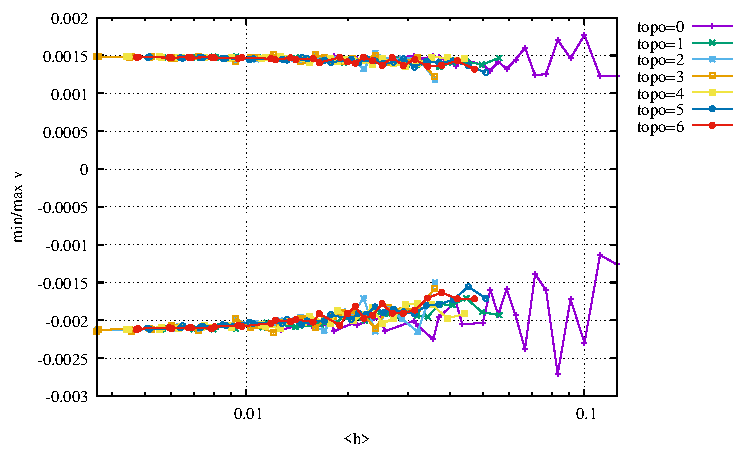
\includegraphics[width=5cm]{python_codes/fieldstone_78/results/stats_v_exp3.pdf}\\
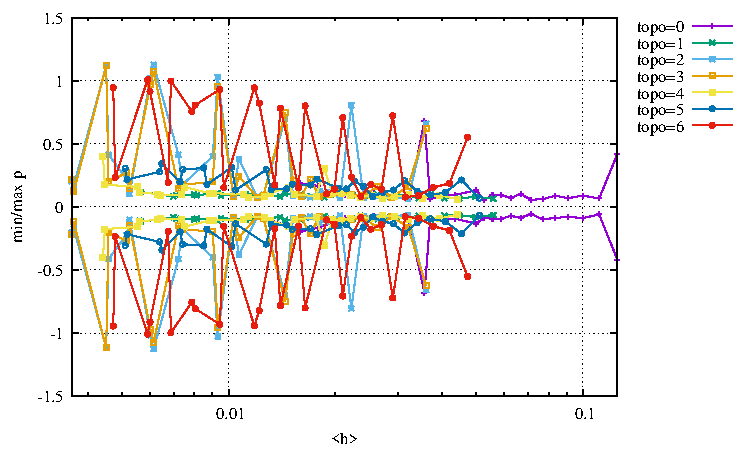
\includegraphics[width=5cm]{python_codes/fieldstone_78/results/stats_p_exp3.pdf}
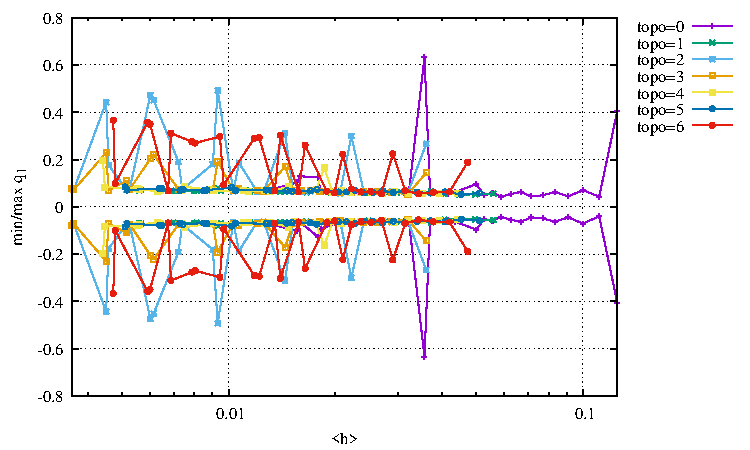
\includegraphics[width=5cm]{python_codes/fieldstone_78/results/stats_q1_exp3.pdf}
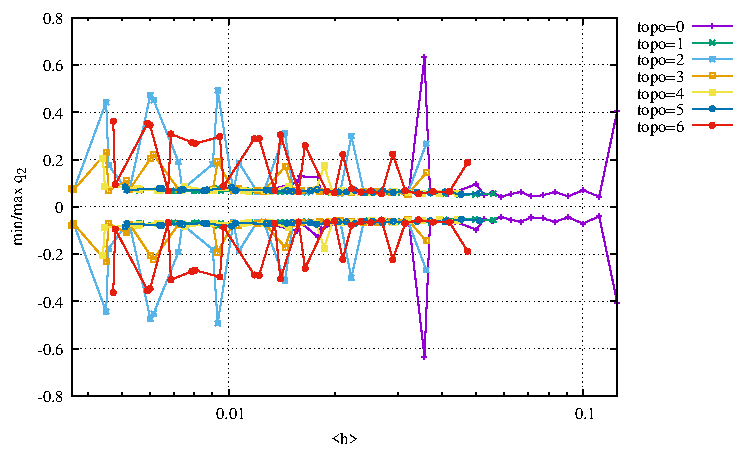
\includegraphics[width=5cm]{python_codes/fieldstone_78/results/stats_q2_exp3.pdf}
\end{center}

\begin{center}
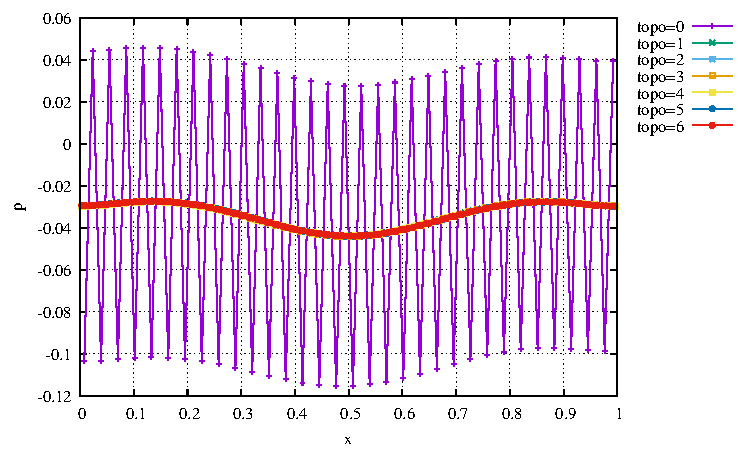
\includegraphics[width=5cm]{python_codes/fieldstone_78/results/pressure_top_exp3.pdf}
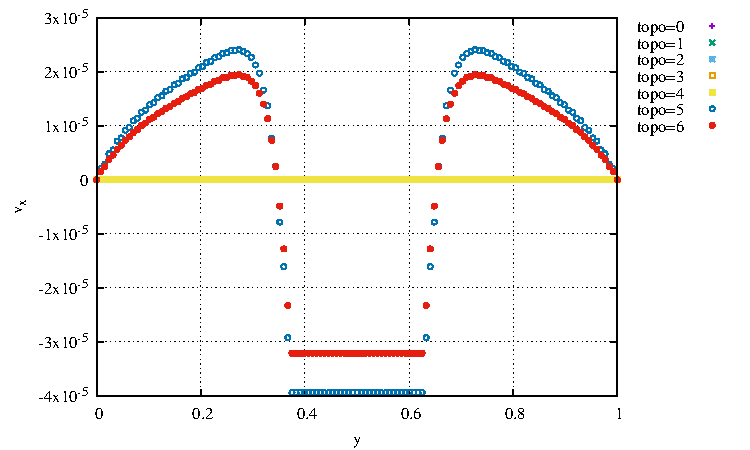
\includegraphics[width=5cm]{python_codes/fieldstone_78/results/vx_profile_exp3.pdf}
\includegraphics[width=5cm]{python_codes/fieldstone_78/results/vy_profile_exp3.pdf}\\
{\captionfont Left: Pressure at the surface; Middle, Right: velocity on vertical line in the middle.}
\end{center}





\newpage
%-------------------------------------------------------------
\subsection*{Experiment 4: The aquarium (EXP)}

{\color{red} description}
Technically a manufactured solution, with $\vec{\upnu}=0$ and $p=\rho g (L_y-y)$.

\begin{center}
\includegraphics[width=5cm]{python_codes/fieldstone_78/results/vrms_exp4.pdf} 
\includegraphics[width=5cm]{python_codes/fieldstone_78/results/stats_u_exp4.pdf}
\includegraphics[width=5cm]{python_codes/fieldstone_78/results/stats_v_exp4.pdf}\\
\includegraphics[width=5cm]{python_codes/fieldstone_78/results/stats_p_exp4.pdf}
\includegraphics[width=5cm]{python_codes/fieldstone_78/results/stats_q1_exp4.pdf}
\includegraphics[width=5cm]{python_codes/fieldstone_78/results/stats_q2_exp4.pdf}
\end{center}

We see that the Stenberg macro-element is the best, with the lowest velocity and pressure errors.

\begin{center}
\includegraphics[width=5cm]{python_codes/fieldstone_78/results/pressure_top_exp4.pdf}
\includegraphics[width=5cm]{python_codes/fieldstone_78/results/vx_profile_exp4.pdf}
\includegraphics[width=5cm]{python_codes/fieldstone_78/results/vy_profile_exp4.pdf}\\
{\captionfont Left: Pressure at the surface; Middle, Right: velocity on vertical line in the middle.}
\end{center}





\newpage
%-------------------------------------------------------------
\subsection*{Experiment 5: SolKz (MS)}

{\color{red} description}

\begin{center}
\includegraphics[width=4cm]{python_codes/fieldstone_78/results/exp05/vel}
\includegraphics[width=4cm]{python_codes/fieldstone_78/results/exp05/p}
\includegraphics[width=4cm]{python_codes/fieldstone_78/results/exp05/by}
\includegraphics[width=4cm]{python_codes/fieldstone_78/results/exp05/eta}\\
{\captionfont Stenberg, 64x64.}
\end{center}


\begin{center}
\includegraphics[width=5cm]{python_codes/fieldstone_78/results/errors_u_exp5.pdf}
\includegraphics[width=5cm]{python_codes/fieldstone_78/results/vrms_exp5.pdf} \\
\includegraphics[width=5cm]{python_codes/fieldstone_78/results/errors_p_exp5.pdf}
\includegraphics[width=5cm]{python_codes/fieldstone_78/results/errors_q1_exp5.pdf}
\includegraphics[width=5cm]{python_codes/fieldstone_78/results/errors_q2_exp5.pdf}\\
\includegraphics[width=5cm]{python_codes/fieldstone_78/results/stats_u_exp5.pdf}
\includegraphics[width=5cm]{python_codes/fieldstone_78/results/stats_v_exp5.pdf}\\
\includegraphics[width=5cm]{python_codes/fieldstone_78/results/stats_p_exp5.pdf}
\includegraphics[width=5cm]{python_codes/fieldstone_78/results/stats_q1_exp5.pdf}
\includegraphics[width=5cm]{python_codes/fieldstone_78/results/stats_q2_exp5.pdf}
\end{center}

\begin{center}
\includegraphics[width=5cm]{python_codes/fieldstone_78/results/pressure_top_exp5.pdf}
\includegraphics[width=5cm]{python_codes/fieldstone_78/results/vx_profile_exp5.pdf}
\includegraphics[width=5cm]{python_codes/fieldstone_78/results/vy_profile_exp5.pdf}\\
{\captionfont Left: Pressure at the surface; Middle, Right: velocity on vertical line in the middle.}
\end{center}

plot analytical pressure and velocity against these!!

\begin{center}
\includegraphics[width=5cm]{python_codes/fieldstone_78/results/mms_solkz/errors_V}
\includegraphics[width=5cm]{python_codes/fieldstone_78/results/mms_solkz/errors_P}
\includegraphics[width=5cm]{python_codes/fieldstone_78/results/mms_solkz/errors_Q} 
\end{center}





\newpage
%-------------------------------------------------------------
\subsection*{Experiment 6: Regularised Lid driven cavity (EXP)}

{\color{red} description}
Domain is 1x1. Viscosity is 1 and density is zero. 
No-slip prescribed at sides and bottom and $\vec{\upnu}=(16x^2(1-x^2),0)$ prescribed on the top.

\begin{center}
\includegraphics[width=5cm]{python_codes/fieldstone_78/results/exp06/vel}
\includegraphics[width=5cm]{python_codes/fieldstone_78/results/exp06/p}\\
{\captionfont Stenberg, 64x64.}
\end{center}

\begin{center}
\includegraphics[width=5cm]{python_codes/fieldstone_78/results/vrms_exp6.pdf} 
\includegraphics[width=5cm]{python_codes/fieldstone_78/results/stats_u_exp6.pdf}
\includegraphics[width=5cm]{python_codes/fieldstone_78/results/stats_v_exp6.pdf}\\
\includegraphics[width=5cm]{python_codes/fieldstone_78/results/stats_p_exp6.pdf}
\includegraphics[width=5cm]{python_codes/fieldstone_78/results/stats_q1_exp6.pdf}
\includegraphics[width=5cm]{python_codes/fieldstone_78/results/stats_q2_exp6.pdf}
\end{center}

pressure of topo 0 is 10**12 , no in plot

\begin{center}
\includegraphics[width=5cm]{python_codes/fieldstone_78/results/pressure_top_exp6.pdf}
\includegraphics[width=5cm]{python_codes/fieldstone_78/results/vx_profile_exp6.pdf}
\includegraphics[width=5cm]{python_codes/fieldstone_78/results/vy_profile_exp6.pdf}\\
{\captionfont Left: Pressure at the surface; Middle, Right: velocity on vertical line in the middle.}
\end{center}








\newpage
%-------------------------------------------------------------
\subsection*{Experiment 7: cavity (MS)}

{\color{red} description}

$eta=1$, 
\[
b_x=0 \qquad b_y=-(8x-2)
\]
\[
u=(2y-1)x(1-x)
\qquad
v=-(2x-1)y(1-y)
\qquad
p=2x(1-2y)
\]
Analytical solution is prescribed on all four sides.

\begin{center}
\includegraphics[width=5cm]{python_codes/fieldstone_78/results/errors_u_exp7.pdf}
\includegraphics[width=5cm]{python_codes/fieldstone_78/results/vrms_exp7.pdf} \\
\includegraphics[width=5cm]{python_codes/fieldstone_78/results/errors_p_exp7.pdf}
\includegraphics[width=5cm]{python_codes/fieldstone_78/results/errors_q1_exp7.pdf}
\includegraphics[width=5cm]{python_codes/fieldstone_78/results/errors_q2_exp7.pdf}\\
\includegraphics[width=5cm]{python_codes/fieldstone_78/results/stats_u_exp7.pdf}
\includegraphics[width=5cm]{python_codes/fieldstone_78/results/stats_v_exp7.pdf}\\
\includegraphics[width=5cm]{python_codes/fieldstone_78/results/stats_p_exp7.pdf}
\includegraphics[width=5cm]{python_codes/fieldstone_78/results/stats_q1_exp7.pdf}
\includegraphics[width=5cm]{python_codes/fieldstone_78/results/stats_q2_exp7.pdf}
\end{center}

\begin{center}
\includegraphics[width=5cm]{python_codes/fieldstone_78/results/pressure_top_exp7.pdf}
\includegraphics[width=5cm]{python_codes/fieldstone_78/results/vx_profile_exp7.pdf}
\includegraphics[width=5cm]{python_codes/fieldstone_78/results/vy_profile_exp7.pdf}\\
{\captionfont Left: Pressure at the surface; Middle, Right: velocity on vertical line in the middle.}
\end{center}




\newpage
%-------------------------------------------------------------
\subsection*{Experiment 8: Earth-sized sinking block (EXP)}

Earth dimensions. 

\begin{center}
\includegraphics[width=5cm]{python_codes/fieldstone_78/results/exp08/vel}
\includegraphics[width=5cm]{python_codes/fieldstone_78/results/exp08/p}
\includegraphics[width=5cm]{python_codes/fieldstone_78/results/exp08/eta}\\
{\captionfont Stenberg, 64x64.}
\end{center}




\newpage
%-------------------------------------------------------------
\subsection*{Experiment 9: Dohrmann \& Bochev (MS)}

It is described in Section~\ref{MMS-mms_dobo}. 
This benchmark is also used in Worthen \etal \cite{wosp14} and Lamichhane \etal \cite{lami17}.
It is for a unit square with $\nu=\eta/\rho=1$ and the smooth exact solution is
\begin{eqnarray}
u(x,y) &=& x+x^2 - 2xy+x^3 - 3xy^2 + x^2y \\
v(x,y) &=& -y-2xy+y^2 -3x^2y + y^3 - xy^2 \\
p(x,y) &=& xy+x+y+x^3y^2 - 4/3
\end{eqnarray}
Note that the pressure field is such that $\int_{\Omega} p \; dV = 0$.


\begin{center}
\includegraphics[width=5cm]{python_codes/fieldstone_78/results/errors_u_exp9.pdf}
\includegraphics[width=5cm]{python_codes/fieldstone_78/results/vrms_exp9.pdf} \\
\includegraphics[width=5cm]{python_codes/fieldstone_78/results/errors_p_exp9.pdf}
\includegraphics[width=5cm]{python_codes/fieldstone_78/results/errors_q1_exp9.pdf}
\includegraphics[width=5cm]{python_codes/fieldstone_78/results/errors_q2_exp9.pdf}\\
\includegraphics[width=5cm]{python_codes/fieldstone_78/results/stats_u_exp9.pdf}
\includegraphics[width=5cm]{python_codes/fieldstone_78/results/stats_v_exp9.pdf}\\
\includegraphics[width=5cm]{python_codes/fieldstone_78/results/stats_p_exp9.pdf}
\includegraphics[width=5cm]{python_codes/fieldstone_78/results/stats_q1_exp9.pdf}
\includegraphics[width=5cm]{python_codes/fieldstone_78/results/stats_q2_exp9.pdf}
\end{center}





\newpage
%-------------------------------------------------------------
\subsection*{Experiment 10: flow around square cylinder (EXP)}

This experiment is inspired by the very common one found in CFD: a laminar flow 
is forced to go around a cylinder (circular or square cross section) often 
generating turbulence in its wake for high-enough Reynolds number Navier-Stokes flow.

The domain is 4x1. Free slip boundary conditions are imposed top and bottom. 
A horizontal flow $\vec{v}=(0,1)$ is prescribed on the left boundary, and the 
right boundary is left open. All the nodes on a square centered in the middle of the domain 
of size 0.125x0.125 are set to no-slip boundary conditions.
Viscosity is one and gravity is switched off.

\begin{center}
\includegraphics[width=5cm]{python_codes/fieldstone_78/results/exp10/vel}
\includegraphics[width=5cm]{python_codes/fieldstone_78/results/exp10/p}
\end{center}

\begin{center}
\includegraphics[width=5cm]{python_codes/fieldstone_78/results/vrms_exp10.pdf} 
\includegraphics[width=5cm]{python_codes/fieldstone_78/results/stats_u_exp10.pdf}
\includegraphics[width=5cm]{python_codes/fieldstone_78/results/stats_v_exp10.pdf}\\
\includegraphics[width=5cm]{python_codes/fieldstone_78/results/stats_p_exp10.pdf}
\includegraphics[width=5cm]{python_codes/fieldstone_78/results/stats_q1_exp10.pdf}
\includegraphics[width=5cm]{python_codes/fieldstone_78/results/stats_q2_exp10.pdf}
\end{center}




\newpage
%-------------------------------------------------------------
\subsection*{Experiment 11: flow over cavity (EXP)}

The domain is 4x1. No slip boundary conditions are imposed on all walls.
The cavity is formed by prescribing $\vec{\upnu}=\vec{0}$ on the right
nodes inside the domain. $\vec{\upnu}=-(y-L_y)(y-L_y/2)$ is prescribed 
on the left inflow boundary while $\upnu_y=0$ is prescribed on the outflow boundary.
Viscosity is one and gravity is switched off.
 
\begin{center}
\includegraphics[width=5cm]{python_codes/fieldstone_78/results/exp11/vel}
\includegraphics[width=5cm]{python_codes/fieldstone_78/results/exp11/p}
\end{center}

\begin{center}
\includegraphics[width=5cm]{python_codes/fieldstone_78/results/vrms_exp11.pdf} 
\includegraphics[width=5cm]{python_codes/fieldstone_78/results/stats_u_exp11.pdf}
\includegraphics[width=5cm]{python_codes/fieldstone_78/results/stats_v_exp11.pdf}\\
\includegraphics[width=5cm]{python_codes/fieldstone_78/results/stats_p_exp11.pdf}
\includegraphics[width=5cm]{python_codes/fieldstone_78/results/stats_q1_exp11.pdf}
\includegraphics[width=5cm]{python_codes/fieldstone_78/results/stats_q2_exp11.pdf}
\end{center}







\newpage
%-------------------------------------------------------------
\subsection*{Experiment 12: flow over obstacle (EXP)}

Domain is 4x1. Viscosity is 1, $rho g = -1$. Free slip top and bottom.
Obstacle is no slip and is composed of nodes at $x=L_x/2$ and $y\le L_y/2$.
$\vec\upnu=(1,0)$ prescribed on the left, $\upnu_y=0$ on the right.

\begin{center}
\includegraphics[width=5cm]{python_codes/fieldstone_78/results/exp12/vel}
\includegraphics[width=5cm]{python_codes/fieldstone_78/results/exp12/p}
\end{center}

\begin{center}
\includegraphics[width=5cm]{python_codes/fieldstone_78/results/vrms_exp12.pdf} 
\includegraphics[width=5cm]{python_codes/fieldstone_78/results/stats_u_exp12.pdf}
\includegraphics[width=5cm]{python_codes/fieldstone_78/results/stats_v_exp12.pdf}\\
\includegraphics[width=5cm]{python_codes/fieldstone_78/results/stats_p_exp12.pdf}
\includegraphics[width=5cm]{python_codes/fieldstone_78/results/stats_q1_exp12.pdf}
\includegraphics[width=5cm]{python_codes/fieldstone_78/results/stats_q2_exp12.pdf}
\end{center}







\newpage
%-------------------------------------------------------------
\subsection*{Experiment 13: solcx (MS)}

\begin{center}
\includegraphics[width=5cm]{python_codes/fieldstone_78/results/errors_u_exp13.pdf}
\includegraphics[width=5cm]{python_codes/fieldstone_78/results/vrms_exp13.pdf} \\
\includegraphics[width=5cm]{python_codes/fieldstone_78/results/errors_p_exp13.pdf}
\includegraphics[width=5cm]{python_codes/fieldstone_78/results/errors_q1_exp13.pdf}
\includegraphics[width=5cm]{python_codes/fieldstone_78/results/errors_q2_exp13.pdf}\\
\includegraphics[width=5cm]{python_codes/fieldstone_78/results/stats_u_exp13.pdf}
\includegraphics[width=5cm]{python_codes/fieldstone_78/results/stats_v_exp13.pdf}\\
\includegraphics[width=5cm]{python_codes/fieldstone_78/results/stats_p_exp13.pdf}
\includegraphics[width=5cm]{python_codes/fieldstone_78/results/stats_q1_exp13.pdf}
\includegraphics[width=5cm]{python_codes/fieldstone_78/results/stats_q2_exp13.pdf}
\end{center}

Odd number of elements:

\begin{center}
\includegraphics[width=6cm]{python_codes/fieldstone_78/results/mms_solcx/odd/errors_V}
\includegraphics[width=6cm]{python_codes/fieldstone_78/results/mms_solcx/odd/errors_P}\\
\includegraphics[width=6cm]{python_codes/fieldstone_78/results/mms_solcx/odd/errors_Q}
\includegraphics[width=6cm]{python_codes/fieldstone_78/results/mms_solcx/odd/vrms.pdf}
\end{center}

Le Tallec macro-element has vertical line in the middle, so that 
even/odd does not matter, there is always an element edge aligned with x=1/2.



\newpage
%-------------------------------------------------------------
\subsection*{Experiment 14: solvi (MS)}

\begin{center}
\includegraphics[width=5cm]{python_codes/fieldstone_78/results/exp14/vel}
\includegraphics[width=5cm]{python_codes/fieldstone_78/results/exp14/p}
\end{center}


\begin{center}
\includegraphics[width=5cm]{python_codes/fieldstone_78/results/errors_u_exp14.pdf}
\includegraphics[width=5cm]{python_codes/fieldstone_78/results/vrms_exp14.pdf} \\
\includegraphics[width=5cm]{python_codes/fieldstone_78/results/errors_p_exp14.pdf}
\includegraphics[width=5cm]{python_codes/fieldstone_78/results/errors_q1_exp14.pdf}
\includegraphics[width=5cm]{python_codes/fieldstone_78/results/errors_q2_exp14.pdf}\\
\includegraphics[width=5cm]{python_codes/fieldstone_78/results/stats_u_exp14.pdf}
\includegraphics[width=5cm]{python_codes/fieldstone_78/results/stats_v_exp14.pdf}\\
\includegraphics[width=5cm]{python_codes/fieldstone_78/results/stats_p_exp14.pdf}
\includegraphics[width=5cm]{python_codes/fieldstone_78/results/stats_q1_exp14.pdf}
\includegraphics[width=5cm]{python_codes/fieldstone_78/results/stats_q2_exp14.pdf}
\end{center}







\newpage
%%%%%%%%%%%%%%%%%%%%%%%%%%%%%%%%%%%%%%%%%%%%%%%%%%%%%%%%%%%%%%%%%%%%%%%%%%%%%%%%%%%%%%%%%%%%

\section*{Discussion}

Intro starts from conclusion of thba22 about Q1P0

3D?

annulus?

use schur complement solver to show it is stable ?

cmat version ? 

put bc inside each experiment ?

mesh anisotropy

we do not consider penalty formulations (no choice of lambda)

Note that other q projections are available.

is $<h>$ best? smthg fancier ?

remark in Gang Lu paper with Dave, about removing checkerboard mode


I have the feeling results can be different if i impose the
constraint in the matrix like it was at first?


what is the real advantage of such a macro-element? it is LBB stable, so 
iterative solver will work optimally, and the pressure has no checkerboard.
Also the number of non-zeros per line of the matrix is small.  
On the other hand it is anisotropic since the 'diamonds are vertical'. 
Also if one would consider a macro-element as an element, it counts 10 velocity nodes and 5 pressures, 
which makes it much more expensive than a $Q_2\times Q_1$ element of the same size...
We find that toplogy 7 does not yield a stable macroelement, so it will be discarded in 
future tests/experiments.

mention c-n-c smoothing a la Douar

Look in pythoncodes/Gel folder, for nullspace caluclations of macroelements

various stabilisations have been proposed for q1p0. However they invariably 
rely on adding a block in the Stokes matrix \ref{XXXX} or altering the 
linear solver so as to filter the spurious modes. 
We here focus on techniques that only involve a specific mesh topology and 
no other modification.
Furthermode it is the author's experimence that 
macro-elt stabilisations are not compatible with buoyancy driven flow


check \cite{nath93}
